\section{Ćwiczenia 10: 11-V-2017}
\subsection{Zadania domowe A}
\paragraph{A1} Rozważmy dwa łańcuchy Markowa, $L_1$ i $L_2$, których stanami jest pięć zbiorów niezależnych ścieżki na trzech wierzchołkach (jeden zbiór pusty, trzy jednoelementowe i jeden dwuelementowy).
\begin{itemize}
\item Zasady przejścia dla łańcucha $L_1$ są następujące:
\begin{itemize}
\item Mając zbiór niezależny $I$, rzuć moneta.
\item Jeśli wypadł orzeł, to wylosuj jeden z trzech wierzchołków $v$, każdy z jednakowym prawdopodobieństwem. Gdy $v \not \in I$ i $I \cup \{v\}$ jest niezależny, wtedy zamień $I$ na $I \cup \{v\}$; w przeciwnym przypadku zostań w $I$.
\item Jeśli wypadła reszka, to wylosuj jeden z trzech wierzchołków $v$, każdy z jednakowym prawdopodobieństwem. Gdy $v \in I$, wtedy zamień $I$ na $I \setminus v$; w przeciwnym przypadku zostań w $I$.
\end{itemize}
\item  Zasady przejścia dla łańcucha $L_2$ są takie:
\begin{itemize}
\item  Mając zbiór niezależny $I$, rzuć monetą.
\item Jeśli wypadł orzeł i istnieje przynajmniej jeden taki zbiór niezależny $J$, że $J \supset  I$ i $|J \setminus I| = 1$, wybierz losowo jeden z takich zbiorów (każdy z jednakowym prawdopodobieństwem) i zamień $I$ na $J$.
\item Jeśli wypadła reszka i istnieje przynajmniej jeden taki zbiór niezależny $J$, że $J \subset I$ i $|I \setminus J| = 1$, wybierz losowo jeden z takich zbiorów (każdy z jednakowym prawdopodobieństwem) i zamień $I$ na $J$.
\item W pozostałych przypadkach zostań w $I$.
\end{itemize}
\end{itemize}
\begin{enumerate}[label=\alph*)]
\item Oceń intuicyjnie, czy rozkłady stacjonarne dla $L_1$ i $L_2$ są takie same.
\begin{comment}
\begin{multicols}{2}
[Oznaczenia: Moneta - $\rightarrow$ rzut monetą\\
O $\rightarrow$  Orzeł, R $\rightarrow$ Reszka\\
ind. $\rightarrow$ niezależny]
% Define block styles
\tikzstyle{decision} = [diamond, draw, text badly centered, node distance=2cm, inner sep=0pt]
\tikzstyle{block} = [rectangle, draw, text centered, rounded corners, minimum height=1em,node distance=2.5cm]
\tikzstyle{line} = [draw,->,ultra thick]
Pierwszy\\
\begin{tikzpicture}
\node[block] (init) {I};
\node[decision, below of=init] (moneta) {Mon};
\node[block, below left of=moneta,text width=5em] (or) {O\newline $\exists _J J\supset I \land |J\setminus I|=1$};
\node[block, below right of=moneta,text width=7em] (re) {R\newline $\exists _J J \text{ind. } \land J\subset I \land |I\setminus J|=1$};
\node[block, left of=init] (or2) {$I:=J$};
\node[block, right of=init] (re2) {$I:=J$};

\path[line] (init) -- (moneta);
\path[line] (moneta) -- (or);
\path[line] (moneta) -- (re);
\path[line] (moneta) -- node [left,near start] {$\sfrac{1}{2}$} (or);
\path[line] (moneta) -- node [right,near start] {$\sfrac{1}{2}$} (re);
\path[line] (or) -- node [left,near start] {tak} (or2);
\path[line] (re) -- node [right,near start] {tak} (re2);
\path[line] (or2) -- (init);
\path[line] (re2) -- (init);
\end{tikzpicture}

Drugi\\
\begin{tikzpicture}
\node[block] (init) {I};
\node[decision, below of=init] (moneta) {Mon};
\node[decision, below left of=moneta,text width=1em] (or) {O: $v$};
\node[decision, below right of=moneta,text width=1em] (re) {R: $v$};
\node[block, below of=or] (or2) {$v\not\in I \land I\cup \{v\} \text{ind. }$};
\node[block, below of=re] (re2) {$v\in I$};
\node[block, left of=init] (or3) {$I:= I\cup \{v\}$};
\node[block, right of=init] (re3) {$I:= I\setminus \{v\}$};

\path[line] (init) -- (moneta);
\path[line] (moneta) -- (or);
\path[line] (moneta) -- (re);
\path[line] (moneta) -- node [left,near start] {$\sfrac{1}{2}$} (or);
\path[line] (moneta) -- node [right,near start] {$\sfrac{1}{2}$} (re);
\path[line] (or) -- node [left,near start] {$\sfrac{1}{3}$} (or2);
\path[line] (re) -- node [right,near start] {$\sfrac{1}{3}$} (re2);
\path[draw,->,bend left,ultra thick] (re2) node [near start] {tak} (re3);
\path[line] (or2) -- node [near start] {tak} (or3);
\path[line] (re2) -- node [near start] {nie} (init);
\path[line] (or2) -- node [near start] {nie} (init);
\path[line] (or3) -- (init);
\path[line] (re3) -- (init);
\end{tikzpicture}
\end{multicols}
\end{comment}

Nie, nie są gdyż są inne warunki przejścia itp.

\item Sprawdź swoje przypuszczenie, budując macierze przejścia i licząc rozkłady stacjonarne dla obu łańcuchów.

\textbf{Ile zbiorów tyle stanów!!}
\begin{figure}[H]
\centering
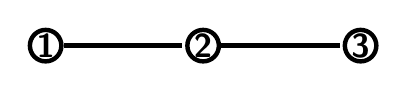
\begin{tikzpicture}[shorten >=1pt, auto, node distance=3cm, ultra thick,main node/.style={circle,draw,minimum size=.4cm,inner sep=0pt}]
\begin{scope}[every node/.style={font=\sffamily\large\bfseries}]
\node [main node](v1) at (0,0) {1};
\node [main node](v2) at (2,0) {2};
\node [main node](v3) at (4,0) {3};
\end{scope}
\path 
	(v1) edge (v2)
    (v2) edge (v3)
         ;
\end{tikzpicture}
\end{figure}
Ważne słowo - \textbf{niezależny} czyli bez połączeń krawędziami!\\
Stany $S=\{\{\emptyset\},\{\emptyset,1\},\{\emptyset,2\},\{\emptyset,3\},\{\emptyset,1,3\} \}$
\begin{enumerate}
\item $L_1$
\begin{align*}
\{\emptyset\}\rightarrow \{\emptyset\} &=\frac{1}{2} &&\text{Reszka potem 1,2,3}\\
\{\emptyset\}\rightarrow \{1\} &=\frac{1}{2}*\frac{1}{3}=\frac{1}{6} &&\text{Orzeł potem 1}\\
\{\emptyset\}\rightarrow \{2\} &=\frac{1}{2}*\frac{1}{3}=\frac{1}{6} &&\text{Orzeł potem 2}\\
\{\emptyset\}\rightarrow \{3\} &=\frac{1}{2}*\frac{1}{3}=\frac{1}{6} &&\text{Orzeł potem 3}\\
\{\emptyset\}\rightarrow \{1,3\} &=0 &&\text{Nie da się}\\
\{1\}\rightarrow \{\emptyset\} &= \frac{1}{2}*\frac{1}{3}=\frac{1}{6}&&\text{Reszka potem 1}\\
\{1\}\rightarrow \{1\} &= \frac{1}{2}*\frac{2}{3}+\frac{1}{2}*\frac{2}{3}=\frac{2}{3}&&\text{Orzeł potem 1,2 i Reszka potem 2,3}\\
\{1\}\rightarrow \{2\} &= 0&&\text{Nie da się}\\
\{1\}\rightarrow \{3\} &= 0&&\text{Nie da się}\\
\{1\}\rightarrow \{1,3\} &= \frac{1}{2}*\frac{1}{3}=\frac{1}{6} &&\text{Orzeł potem 3}\\
\{2\}\rightarrow \{\emptyset\} &= \frac{1}{2}*\frac{1}{3}=\frac{1}{6} &&\text{Reszka potem 2}\\
\{2\}\rightarrow \{1\} &= 0&&\text{Nie da się}\\
\{2\}\rightarrow \{2\} &= \frac{1}{2}*\frac{3}{3}+\frac{1}{2}*\frac{2}{3}=\frac{5}{6}&&\text{Orzeł potem 1,2,3 i Reszka potem 1,3}\\
\{2\}\rightarrow \{3\} &=0 &&\text{Nie da się}\\
\{2\}\rightarrow \{1,3\} &=0 &&\text{Nie da się}\\
\{3\}\rightarrow \{\emptyset\} &=\frac{1}{2}*\frac{1}{3}=\frac{1}{6} &&\text{Reszka potem 3}\\
\{3\}\rightarrow \{1\} &=0 &&\text{Nie da się}\\
\{3\}\rightarrow \{2\} &=0 &&\text{Nie da się}\\
\{3\}\rightarrow \{3\} &=\frac{1}{2}*\frac{2}{3}+\frac{1}{2}*\frac{2}{3}=\frac{2}{3} &&\text{Orzeł potem 2,3 i Reszka potem 1,2}\\
\{3\}\rightarrow \{1,3\} &=\frac{1}{2}*\frac{1}{3}=\frac{1}{6} &&\text{Orzeł potem 1}\\
\{1,3\}\rightarrow \{\emptyset\} &=0 &&\text{Nie da się}\\
\{1,3\}\rightarrow \{1\} &=\frac{1}{2}*\frac{1}{3}=\frac{1}{6} &&\text{Reszka potem 3}\\
\{1,3\}\rightarrow \{2\} &=0 &&\text{Nie da się}\\
\{1,3\}\rightarrow \{3\} &=\frac{1}{2}*\frac{1}{3}=\frac{1}{6} &&\text{Reszka potem 1}\\
\{1,3\}\rightarrow \{1,3\} &=\frac{1}{2}*\frac{3}{3}+\frac{1}{2}*\frac{1}{3} = \frac{4}{6}&&\text{Orzeł potem 1,2,3 i Reszka potem 2}
\end{align*}
\begin{figure}[H]
\centering
\begin{tikzpicture}[shorten >=1pt, auto, node distance=3cm, ultra thick,main node/.style={circle,draw,minimum size=.6cm,inner sep=0pt}]
\begin{scope}[every node/.style={font=\sffamily\large\bfseries}]
\node [main node](v1) at (3,0) {$\{\emptyset\}$};
\node [main node](v2) at (0,-1) {$\{1\}$};
\node [main node](v3) at (4,2) {$\{2\}$};
\node [main node](v4) at (-2.5,2) {$\{3\}$};
\node [main node](v5) at (-1,3) {$\{1,3\}$};
\end{scope}
\path 
	(v1) edge [loop below] node {$\sfrac{1}{2}$} (v1)
    	 edge [->,bend left] node[near start] {$\sfrac{1}{6}$} (v2)
         edge [->,bend left] node[near start] {$\sfrac{1}{6}$} (v3)
         edge [->,bend left] node[near start] {$\sfrac{1}{6}$} (v4)
    (v2) edge [loop left] node {$\sfrac{2}{3}$} (v2)
    	 edge [->,bend left] node[near start] {$\sfrac{1}{6}$} (v1)
         edge [->,bend left] node[near start] {$\sfrac{1}{6}$} (v5)
    (v3) edge [loop right] node {$\sfrac{5}{6}$} (v3)
    	 edge [->,bend left] node[near start] {$\sfrac{1}{6}$} (v1)
    (v4) edge [loop left] node {$\sfrac{2}{3}$} (v4)
    	 edge [->] node[near start] {$\sfrac{1}{6}$} (v1)
         edge [->,bend left] node[near start] {$\sfrac{1}{6}$} (v5)
    (v5) edge [->,bend left] node[near start] {$\sfrac{1}{6}$} (v1)
         edge [->,bend left] node[near start] {$\sfrac{1}{6}$} (v3)
         edge [->,bend left] node[near start] {$\sfrac{2}{3}$} (v4)
         ;
\end{tikzpicture}
\end{figure}
$$\mathbb{P}_{L_1}=\bbordermatrix{
&\{\emptyset\}&\{1\}&\{2\}&\{3\}&\{1,3\} \cr
\{\emptyset\} & \sfrac{1}{2} & \sfrac{1}{6} & \sfrac{1}{6} & \sfrac{1}{6} & 0 \cr
\{1\} & \sfrac{1}{6} & \sfrac{2}{3} & 0 & 0 & \sfrac{1}{6}  \cr
\{2\} & \sfrac{1}{6} & 0 & \sfrac{5}{6} & 0 & 0  \cr
\{3\} & \sfrac{1}{6} & 0 & 0 & \sfrac{2}{3} & \sfrac{1}{6}  \cr
\{1,3\} & 0 & \sfrac{1}{6} & 0 & \sfrac{1}{6} & \sfrac{4}{6} \cr
}$$
Rozkład stacjonarny:
\begin{align*}
&\bar{\pi}\mathbb{P}_{L_1}=\bar{\pi}\\
&\left[\pi _1,\pi _2,\pi _3,\pi _4,\pi _5,\right]\begin{bmatrix}
\sfrac{1}{2} & \sfrac{1}{6} & \sfrac{1}{6} & \sfrac{1}{6} & 0\\
\sfrac{1}{6} & \sfrac{2}{3} & 0 & 0 & \sfrac{1}{6}  \\
\sfrac{1}{6} & 0 & \sfrac{5}{6} & 0 & 0  \\
\sfrac{1}{6} & 0 & 0 & \sfrac{2}{3} & \sfrac{1}{6}  \\
0 & \sfrac{1}{6} & 0 & \sfrac{1}{6} & \sfrac{4}{6}
\end{bmatrix}=\left[\pi _1,\pi _2,\pi _3,\pi _4,\pi _5,\right]\\
&\left\{\begin{matrix}
\frac{1}{2} \pi _1+\frac{1}{6} \pi_2+\frac{1}{6} \pi _3 +\frac{1}{6} \pi _4 &= \pi _1\\
\frac{1}{6} \pi _1+\frac{2}{3} \pi _2+\frac{1}{6} \pi _5 &= \pi _2\\
\frac{1}{6} \pi _1+\frac{5}{6} \pi _3 &= \pi _3\\
\frac{1}{6} \pi _1+\frac{2}{3} \pi _4+\frac{1}{6} \pi _5 &= \pi _4\\
\frac{1}{6} \pi _2+\frac{1}{6} \pi _4+\frac{2}{3} \pi _5 &= \pi _5
\end{matrix}\right. \Leftrightarrow \left\{\begin{matrix}
\frac{1}{6} \pi_2+\frac{1}{6} \pi _3 +\frac{1}{6} \pi _4 & = \frac{1}{2}\pi _ 1\\
\frac{1}{6} \pi _1+\frac{1}{6} \pi _5 &= \frac{1}{3}\pi _2\\
\frac{1}{6} \pi _1&=\frac{1}{6} \pi _3\\
\frac{1}{6} \pi _1+\frac{1}{6} \pi _5 &=\frac{1}{3} \pi _4\\
\frac{1}{6} \pi _2+\frac{1}{6} \pi _4 &= \frac{1}{3}\pi _5
\end{matrix}\right. \Leftrightarrow \\
&\Leftrightarrow \left\{\begin{matrix}
\pi _1 &= \pi _2\\
\pi _1 &= \pi _3\\
\pi _1 &= \pi _4 \\
\pi _1 &= \pi _5 
\end{matrix}\right.\\
&\pi _1+\pi _2+\pi _3+\pi _4+\pi _5=1\Leftrightarrow 5\pi _1 = 1 \Leftrightarrow \pi _1 = \frac{1}{5}\\
&\bar{\pi}=\left[\frac{1}{5},\frac{1}{5},\frac{1}{5},\frac{1}{5},\frac{1}{5}\right]
\end{align*}

\item $L_2$\\
\textbf{Uwaga!} zbiór pusty jest podzbiorem dowolnego zbioru\\
Pamiętajmy, że $\{1\} \subset \{1\}$\\
Stany $S=\{\{\emptyset\},\{\emptyset,1\},\{\emptyset,2\},\{\emptyset,3\},\{\emptyset,1,3\} \}$

\begin{align*}
\{\emptyset\}\rightarrow \{\emptyset\} &= \frac{1}{2} &&\text{Reszka}\\
\{\emptyset\}\rightarrow \{1\} &= \frac{1}{2}*\frac{1}{3}=\frac{1}{6} &&\text{Orzeł potem zbiór 1 (z trzech)}\\
\{\emptyset\}\rightarrow \{2\} &= \frac{1}{2}*\frac{1}{3}=\frac{1}{6}&&\text{Orzeł potem zbiór 2 (z trzech)}\\
\{\emptyset\}\rightarrow \{3\} &= \frac{1}{2}*\frac{1}{3}=\frac{1}{6}&&\text{Orzeł potem zbiór 3 (z trzech)}\\
\{\emptyset\}\rightarrow \{1,3\} &= 0 &&\text{Zdarzenie niemożliwe}\\
\{1\}\rightarrow \{\emptyset\} &= \frac{1}{2}*1=\frac{1}{2} &&\text{Reszka potem zbiór 0 }\\
\{1\}\rightarrow \{1\} &=0 &&\text{Nie spełnia warunków Orła i Reszki}\\
\{1\}\rightarrow \{2\} &=0 &&\text{Nie spełnia warunków Orła i Reszki}\\
\{1\}\rightarrow \{3\} &=0 &&\text{Nie spełnia warunków Orła i Reszki}\\
\{1\}\rightarrow \{1,3\} &= \frac{1}{2}*1=\frac{1}{2}&&\text{Orzeł potem zbiór 1,3}\\
\{2\}\rightarrow \{\emptyset\} &=\frac{1}{2}*1=\frac{1}{2} &&\text{Reszka potem zbiór pusty}\\
\{2\}\rightarrow \{1\} &=0 &&\text{Zdarzenie niemożliwe}\\
\{2\}\rightarrow \{2\} &=\frac{1}{2} &&\text{Orzeł}\\
\{2\}\rightarrow \{3\} &=0 &&\text{Zdarzenie niemożliwe}\\
\{2\}\rightarrow \{1,3\} &=\frac{1}{8} &&\text{Nie spełnia warunków Orła i Reszki}\\
\{3\}\rightarrow \{\emptyset\} &=\frac{1}{2}*1=\frac{1}{2} &&\text{Reszka potem zbiór 0}\\
\{3\}\rightarrow \{1\} &=0 &&\text{Nie spełnia warunków Orła i Reszki}\\
\{3\}\rightarrow \{2\} &=0 &&\text{Nie spełnia warunków Orła i Reszki}\\
\{3\}\rightarrow \{3\} &=0 &&\text{Nie spełnia warunków Orła i Reszki}\\
\{3\}\rightarrow \{1,3\} &=\frac{1}{2}*1=\frac{1}{2} &&\text{Orzeł potem zbiór 1,3}\\
\{1,3\}\rightarrow \{\emptyset\} &=0 &&\text{Nie spełnia warunków Orła i Reszki}\\
\{1,3\}\rightarrow \{1\} &=\frac{1}{2}*1=\frac{1}{2}  &&\text{Reszka potem zbiór 1}\\
\{1,3\}\rightarrow \{2\} &=0 &&\text{Nie spełnia warunków Orła i Reszki}\\
\{1,3\}\rightarrow \{3\} &=\frac{1}{2}*1 &&\text{Reszka potem zbiór 3}\\
\{1,3\}\rightarrow \{1,3\} &=0 &&\text{Nie spełnia warunków Orła i Reszki}
\end{align*}
$$\mathbb{P}_{L_1}=\bbordermatrix{
&\{\emptyset\}&\{1\}&\{2\}&\{3\}&\{1,3\} \cr
\{\emptyset\} & \sfrac{1}{2} & \sfrac{1}{6} & \sfrac{1}{6} & \sfrac{1}{6} & 0 \cr
\{1\} & \sfrac{1}{2} & 0 & 0 & 0 & \sfrac{1}{2} \cr
\{2\} & \sfrac{1}{2} & 0 & \sfrac{1}{2} & 0 & 0  \cr
\{3\} & \sfrac{1}{2} & 0 & 0 & 0 & \sfrac{1}{2} \cr
\{1,3\} & 0 & \sfrac{1}{2} & 0 & \sfrac{1}{2} & 0 \cr
}$$
\begin{figure}[H]
\centering
\begin{tikzpicture}[shorten >=1pt, auto, node distance=3cm, ultra thick,main node/.style={circle,draw,minimum size=.6cm,inner sep=0pt}]
\begin{scope}[every node/.style={font=\sffamily\large\bfseries}]
\node [main node](v1) at (-1,-1.5) {$\{\emptyset\}$};
\node [main node](v2) at (3.5,-1.5) {$\{1\}$};
\node [main node](v3) at (3.5,3.5) {$\{2\}$};
\node [main node](v4) at (-2.5,1.5) {$\{3\}$};
\node [main node](v5) at (-1,3) {$\{1,3\}$};
\end{scope}
\path 
	(v1) edge [loop left] node {$\sfrac{1}{2}$} (v1)
    	 edge [->,bend left] node[near start] {$\sfrac{1}{6}$} (v2)
         edge [->,bend left] node[near start] {$\sfrac{1}{6}$} (v3)
         edge [->,bend left] node[near start] {$\sfrac{1}{6}$} (v4)
    (v2) edge [->,bend left] node[near start] {$\sfrac{1}{2}$} (v1)
         edge [->,bend left] node[near start] {$\sfrac{1}{2}$} (v5)
    (v3) edge [->,bend left] node[near start] {$\sfrac{1}{2}$} (v1)
    	 edge [->,bend left] node[near start] {$\sfrac{1}{2}$} (v3)
    (v4) edge [->,bend left] node[near start] {$\sfrac{1}{2}$} (v1)
         edge [->,bend left] node[near start] {$\sfrac{1}{2}$} (v5)
    (v5) edge [->,bend left] node[near start] {$\sfrac{1}{2}$} (v2)
         edge [->,bend left] node[near start] {$\sfrac{1}{2}$} (v4)
         ;
\end{tikzpicture}
\end{figure}
Rozkład stacjonarny:
\begin{align*}
&\bar{\pi}\mathbb{P}_{L_1}=\bar{\pi}\\
&\left[\pi _1,\pi _2,\pi _3,\pi _4,\pi _5,\right]\begin{bmatrix}
\sfrac{1}{2} & \sfrac{1}{6} & \sfrac{1}{6} & \sfrac{1}{6} & 0 \\
\sfrac{1}{2} & 0 & 0 & 0 & \sfrac{1}{2} \\
\sfrac{1}{2} & 0 & \sfrac{1}{2} & 0 & 0  \\
\sfrac{1}{2} & 0 & 0 & 0 & \sfrac{1}{2} \\
0 & \sfrac{1}{2} & 0 & \sfrac{1}{2} & 0 
\end{bmatrix}=\left[\pi _1,\pi _2,\pi _3,\pi _4,\pi _5,\right]\\
&\left\{\begin{matrix}
\frac{1}{2}\pi _1 + \frac{1}{2}\pi _2+ \frac{1}{2}\pi _3+ \frac{1}{2}\pi _4 &= \pi _1\\
\frac{1}{6}\pi _1 + \frac{1}{2}\pi _5 &= \pi _2\\
\frac{1}{6}\pi _1 + \frac{1}{2}\pi _3 &= \pi _3\\
\frac{1}{6}\pi _1 + \frac{1}{2}\pi _5 &= \pi_4 \\
\frac{1}{2}\pi _2+\frac{1}{2}\pi _4 &= \pi _5
\end{matrix}\right. \Leftrightarrow \left\{\begin{matrix}
\pi _1 &= 3x\\
\pi _2 &= x\\
\pi _3 &= x\\
\pi _4 &= x\\
\pi _5 &= x
\end{matrix}\right.\\
&\bar{\pi}=\left[\frac{3}{7},\frac{1}{7},\frac{1}{7},\frac{1}{7},\frac{1}{7}\right]
\end{align*}
\end{enumerate}
\end{enumerate}



\paragraph{A2} Opisz zwięźle ideę algorytmu, generującego losowy zbiór niezależny w grafie (w tym zbiór pusty) w taki sposób, że \label{par:10-A2}

\begin{enumerate}[label=\alph*)]
\item  w rozkładzie stacjonarnym dla tego procesu wszystkie podzbiory są jednakowo prawdopodobne.

\begin{enumerate}[label=\arabic*.]
\item Startujemy od zbioru pustego $I=\emptyset $
\item Rzucamy monetą taką, że $\mathsf{Pr}(O)=p$ a $\mathsf{Pr}(R)=1-\mathsf{Pr}(O)=1-p$
\item Wybieramy losowo wierzchołek $v$ w grafie $G$,
\item Jeśli 
\begin{itemize}
\item[] wypadł \textbf{O}rzeł i $I=I\cup \{v\}$ jest niezależny to\\
$I:=I\cup \{v\}$
\item[] wypadła \textbf{R}eszka i $v\in I$ to\\
$I:=I- \{v\}$
\end{itemize}
\item wracamy do punktu 2.
\end{enumerate}
\textbf{Odpowiedź: }uzyskamy gdy za $p$ podstawimy $\frac{1}{2}$ - wtedy uzyskamy ergodyczny Łańcuch Markowa - nie jest okresowy i jest nieprzywiedlny.
\begin{figure}[H]
\centering
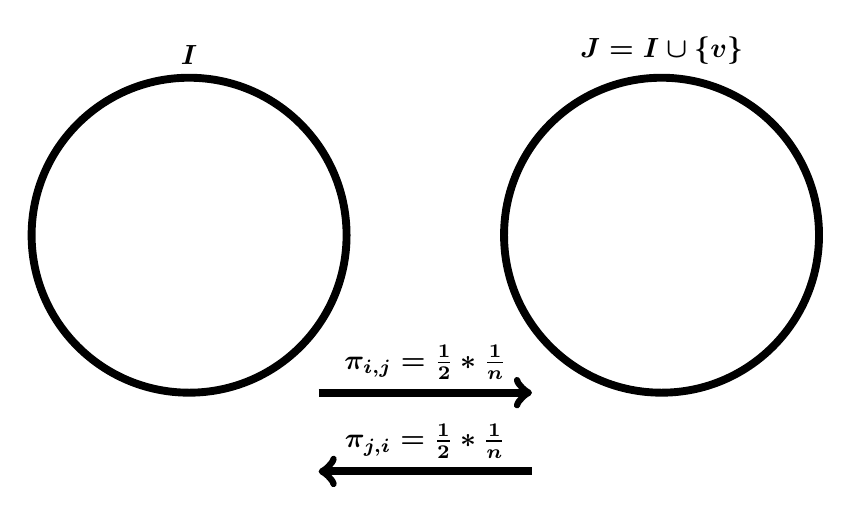
\begin{tikzpicture}[font=\boldmath,ultra thick,]
\draw[solid, line width=1mm]  (0,0) ellipse (2 and 2) node [above=2cm] {$I$};
\draw[solid, line width=1mm]  (6,0) ellipse (2 and 2) node [above=2cm] {$J=I\cup \{v\}$};
\node (v1) at (1.5,-2) {};
\node (v2) at (4.5,-2) {};
\node (v3) at (1.5,-3) {};
\node (v4) at (4.5,-3) {};
\draw[->,solid,line width=1mm,fill=black]  (v1) edge node [above] {$\pi _{i,j}=\frac{1}{2}*\frac{1}{n}$} (v2);
\draw[->,solid,line width=1mm,fill=black]  (v4) edge node [above] {$\pi _{j,i}=\frac{1}{2}*\frac{1}{n}$}(v3);
\end{tikzpicture}
\caption*{$\frac{1}{n}$ $\rightarrow$ wybranie 1 z $n$ wierzchołków\\$\frac{1}{2}$ $\rightarrow$ \textbf{O}rzeł albo \textbf{R}eszka\\Dowód okresowości - można wrócić z każdego stanu $I$ do każdego stanu $J$ i vice versa oraz nieprzywiedlności - z każdego okresu można się dostać w naturalnej liczbie kroków.}
\end{figure}
Więc dla $$\lim _{n\to\infty}\pi _{i,j}(n)=\pi _j$$ Co więcej dla dowolnej pary stanów $i,j\in S$ otrzymujemy $\pi_{i,j}=\pi _{j,i}$ więc $$\bar{\pi}=\left[\frac{1}{|S|},\frac{1}{|S|},...,\frac{1}{|S|}\right]$$

\item po wielu krokach otrzymamy każdy podzbiór niezależny z prawdopodobieństwem w przybliżeniu jednakowym.

\textbf{Odpowiedź: }Analogicznie jak w przykładzie powyżej, jednakże dla $p= \frac{1}{2}$ analogicznie jak wyżej rozkład po wielu ktokach będzie rozkładem stacjonarnym jak w podpunkcie a).
\item w rozkładzie stacjonarnym dla tego procesu każdy ze zbiorów niezależnych $A$ występuje z prawdopodobieństwem, 
$$\frac{2^{|A|}}{\sum _Z2^{|Z|}}$$
gdzie suma w mianowniku przebiega wszystkie zbiory niezależne grafu (w tym zbiór pusty).

\textbf{Odpowiedź: } Zgodnie z modyfikacją algorytmu: 
\begin{enumerate}[label=\arabic*.]
\item Startujemy od zbioru pustego $I=\emptyset $
\item Rzucamy monetą taką, że $\mathsf{Pr}(O)=p$\footnote{prawdopodobieństwo ,,wylosowania'' \textbf{O}rła} a $\mathsf{Pr}(R)=1-\mathsf{Pr}(O)=1-p$\footnote{prawdopodobieństwo ,,wylosowania'' \textbf{R}eszki}
\item Wybieramy losowo wierzchołek $v$ w grafie $G$,
\item Jeśli 
\begin{itemize}
\item[] wypadł \textbf{O}rzeł i $I=I\cup \{v\}$ jest niezależny to\\
$I:=I\cup \{v\}$
\item[] wypadła \textbf{R}eszka i $v\in I$ to\\
$I:=I- \{v\}$
\end{itemize}
\item wracamy do punktu 2.
\end{enumerate}

Szukamy takiego $$\alpha ^I$$


dla $p=\frac{1}{3}, \alpha =2$ 
\begin{align*}
\alpha ^{|I|}\pi_{i,j}&=\alpha ^{|J|}\pi_{j,i}\\
\alpha ^{|I|}p\frac{1}{n}=\alpha ^{|J|}(1-p)\frac{1}{n}&=\alpha *\alpha ^{|I|}(1-p)\frac{1}{n}\\
p&=\alpha (1-p)\\
p&=\alpha -\alpha p\\
p+\alpha p&=\alpha\\
p&=\frac{\alpha}{1+\alpha}
\end{align*}


\item w rozkładzie stacjonarnym dla tego procesu każdy ze zbiorów niezależnych $A$ występuje z prawdopodobieństwem $$\frac{\left(\sfrac{1}{2}\right)^{|A|}}{\sum _Z \left(\sfrac{1}{2}\right)^{|Z|}}$$
gdzie suma w mianowniku przebiega wszystkie zbiory niezależne grafu (w tym zbiór pusty).

\textbf{Odpowiedź: }dla $p=\frac{1}{3}, \alpha =\sfrac{1}{2}$ 
\end{enumerate}
Dokładnie uzasadnij poprawność algorytmu.

\paragraph{A3} Mamy $2$ kolory i graf $G = C_4$, czyli będący cyklem o $4$ wierzchołkach. Generujemy wszystkie właściwe kolorowania wierzchołków grafu G następująco:
\begin{itemize}
\item Mając kolorowanie właściwe, wylosuj jeden z wierzchołków $v$, każdy z jednakowym prawdopodobieństwem i wylosuj jeden z kolorów $i$, każdy z jednakowym prawdopodobieństwem.
\item Jeśli po przemalowaniu wierzchołka $v$ na kolor $i$ kolorowanie pozostaje właściwe, przemaluj $v$ na kolor $i$.
\item W przeciwnym przypadku pozostaw kolorowanie bez zmian.
\end{itemize}
\begin{multicols}{3}
\begin{figure}[H]
\centering
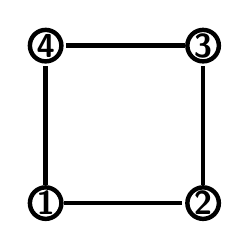
\begin{tikzpicture}[shorten >=1pt, auto, node distance=3cm, ultra thick,main node/.style={circle,draw,minimum size=.4cm,inner sep=0pt}]
\begin{scope}[every node/.style={font=\sffamily\large\bfseries}]
\node [main node](v1) at (0,0) {1};
\node [main node](v2) at (2,0) {2};
\node [main node](v3) at (2,2) {3};
\node [main node](v4) at (0,2) {4};
\end{scope}
\path 
	(v1) edge (v2)
    (v1) edge (v4)
    (v2) edge (v3)
    (v3) edge (v4)
         ;
\end{tikzpicture}
\caption*{$C_4$}
\end{figure}
\begin{figure}[H]
\centering
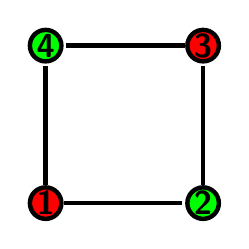
\begin{tikzpicture}[shorten >=1pt, auto, node distance=3cm, ultra thick,main node/.style={circle,draw,minimum size=.4cm,inner sep=0pt}]
\begin{scope}[every node/.style={font=\sffamily\large\bfseries}]
\node [main node,fill=red](v1) at (0,0) {1};
\node [main node,fill=green](v2) at (2,0) {2};
\node [main node,fill=red](v3) at (2,2) {3};
\node [main node,fill=green](v4) at (0,2) {4};
\end{scope}
\path 
	(v1) edge (v2)
    (v1) edge (v4)
    (v2) edge (v3)
    (v3) edge (v4)
         ;
\end{tikzpicture}
\caption*{I ,,Pokolorowane'' $C_4$}
\end{figure}
\begin{figure}[H]
\centering
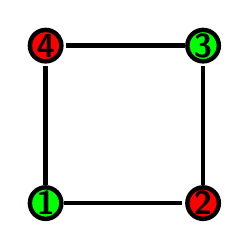
\begin{tikzpicture}[shorten >=1pt, auto, node distance=3cm, ultra thick,main node/.style={circle,draw,minimum size=.4cm,inner sep=0pt}]
\begin{scope}[every node/.style={font=\sffamily\large\bfseries}]
\node [main node,fill=green](v1) at (0,0) {1};
\node [main node,fill=red](v2) at (2,0) {2};
\node [main node,fill=green](v3) at (2,2) {3};
\node [main node,fill=red](v4) at (0,2) {4};
\end{scope}
\path 
	(v1) edge (v2)
    (v1) edge (v4)
    (v2) edge (v3)
    (v3) edge (v4)
         ;
\end{tikzpicture}
\caption*{II ,,Pokolorowane'' $C_4$}
\end{figure}
\end{multicols}
\begin{enumerate}[label=\alph*)]
\item Narysuj graf skierowany, obrazujący łańcuch Markowa odpowiadający podanemu algorytmowi. Zbiorem stanów powinny być wszystkie właściwe kolorowania grafu $G$.
\begin{figure}[H]
\centering
\begin{tikzpicture}[shorten >=1pt, auto, node distance=3cm, ultra thick,main node/.style={rectangle,draw,minimum size=.4cm,text width=3cm,text centered,rounded corners}]
\begin{scope}[every node/.style={font=\sffamily}]
\node (v0) at (-2.5,1.5) {START};
\node [main node](v1) at (0,0) {Wylosuj jeden z wierzchołków $v$};
\node [main node](v2) at (0,-2) {Wylosuj jeden z kolorów $i$};
\node [main node](v3) at (0,-4) {Czy kolorowanie jest właściwe?};
\node [main node](v4) at (-2,-6) {Przemaluj $v$ na $i$};
\node [main node](v5) at (2,-6) {Pozostaw bez zmian};

\end{scope}
\path 
	(v0) edge [->] node {} (v1)
	(v1) edge [->] node {$\sfrac{1}{4}$} (v2)
    (v2) edge [->] node[->] {$\sfrac{1}{2}$} (v3)
    (v3) edge [->] node {TAK} (v4)
    (v3) edge [->] node {NIE} (v5)
         ;
\end{tikzpicture}
\caption*{,,Pokolorowane'' $C_4$}
\end{figure}

Stany: $S:\{\{\text{I Pokolorowanie}\},\{\text{II Pokolorowanie}\}\}$
\begin{figure}[H]
\centering

\begin{tikzpicture}[shorten >=1pt, auto, node distance=3cm, ultra thick,main node/.style={rectangle,draw,minimum size=.4cm,inner sep=0pt}]
\begin{scope}[every node/.style={font=\sffamily}]
\node [main node](v1) at (0,0) {$\{\text{I Pokolorowanie}\}$};
\node [main node](v2) at (4,0) {$\{\text{II Pokolorowanie}\}$};
\end{scope}
\path 
	(v1) edge [loop above] node[near start] {$1$} (v1)
    (v2) edge [loop above] node[near start] {$1$} (v2)
         ;
\end{tikzpicture}
\end{figure}


\item Czy po bardzo dużej liczbie kroków każde właściwe kolorowanie będzie w przybliżeniu jednakowo prawdopodobne, niezależnie jaki był stan początkowy?

\textbf{Odpowiedź:} \textbf{NIE}, gdyż jak widać z rysunku diagramu powyżej, poszczególne stany łańcucha są pochłaniające - czytaj z stanu I nie przejdę do stanu II i vive versa. Czyli po bardzo dużej liczbie kroków prawdopodobieństwo będzie równe prawdopodobieństwu początkowemu. 
\end{enumerate}


\paragraph{A4} Generujemy lasy rozpięte grafu $K_3$ następująco. Zaczynamy od dowolnego lasu rozpiętego, a w każdym kroku, Mając wygenerowany las $H$, wybieramy z jednakowym prawdopodobieństwem jakąś krawędź z $E(K_3)$, a następnie rzucamy symetryczna, monetą.
\begin{figure}[H]
\centering
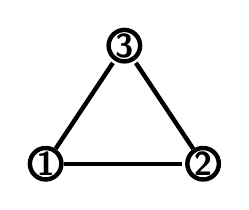
\begin{tikzpicture}[shorten >=1pt, auto, node distance=3cm, ultra thick,main node/.style={circle,draw,minimum size=.4cm,inner sep=0pt}]
\begin{scope}[every node/.style={font=\sffamily\large\bfseries}]
\node [main node](v1) at (0,0) {1};
\node [main node](v2) at (2,0) {2};
\node [main node](v3) at (1,1.5) {3};
\end{scope}
\path 
	(v1) edge (v2)
    (v1) edge (v3)
    (v2) edge (v3)
         ;
\end{tikzpicture}
\caption*{$K_3$}
\end{figure}
\begin{multicols}{4}[Możliwe lasy rozpięte na $K_3$]
Stan $I\ \rightarrow\ S_{I}$:\\
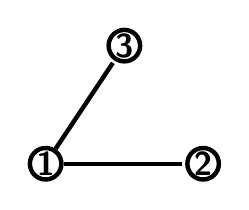
\begin{tikzpicture}[shorten >=1pt, auto, node distance=3cm, ultra thick,main node/.style={circle,draw,minimum size=.4cm,inner sep=0pt}]
\begin{scope}[every node/.style={font=\sffamily\large\bfseries}]
\node [main node](v1) at (0,0) {1};
\node [main node](v2) at (2,0) {2};
\node [main node](v3) at (1,1.5) {3};
\end{scope}
\path 
	(v1) edge (v2)
    (v1) edge (v3)
         ;
\end{tikzpicture}
Stan $II\ \rightarrow\ S_{II}$:\\
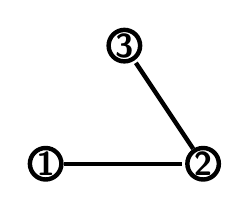
\begin{tikzpicture}[shorten >=1pt, auto, node distance=3cm, ultra thick,main node/.style={circle,draw,minimum size=.4cm,inner sep=0pt}]
\begin{scope}[every node/.style={font=\sffamily\large\bfseries}]
\node [main node](v1) at (0,0) {1};
\node [main node](v2) at (2,0) {2};
\node [main node](v3) at (1,1.5) {3};
\end{scope}
\path 
	(v1) edge (v2)
    (v2) edge (v3)
         ;
\end{tikzpicture}
Stan $III\ \rightarrow\ S_{III}$:\\
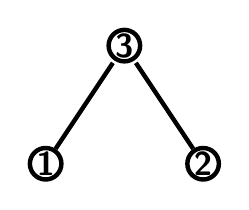
\begin{tikzpicture}[shorten >=1pt, auto, node distance=3cm, ultra thick,main node/.style={circle,draw,minimum size=.4cm,inner sep=0pt}]
\begin{scope}[every node/.style={font=\sffamily\large\bfseries}]
\node [main node](v1) at (0,0) {1};
\node [main node](v2) at (2,0) {2};
\node [main node](v3) at (1,1.5) {3};
\end{scope}
\path 
    (v1) edge (v3)
    (v2) edge (v3)
         ;
\end{tikzpicture}
Stan $IV\ \rightarrow\ S_{IV}$:\\
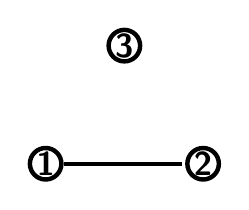
\begin{tikzpicture}[shorten >=1pt, auto, node distance=3cm, ultra thick,main node/.style={circle,draw,minimum size=.4cm,inner sep=0pt}]
\begin{scope}[every node/.style={font=\sffamily\large\bfseries}]
\node [main node](v1) at (0,0) {1};
\node [main node](v2) at (2,0) {2};
\node [main node](v3) at (1,1.5) {3};
\end{scope}
\path 
	(v1) edge (v2)
         ;
\end{tikzpicture}
Stan $V\ \rightarrow\ S_{V}$:\\
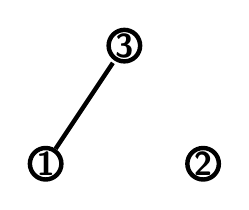
\begin{tikzpicture}[shorten >=1pt, auto, node distance=3cm, ultra thick,main node/.style={circle,draw,minimum size=.4cm,inner sep=0pt}]
\begin{scope}[every node/.style={font=\sffamily\large\bfseries}]
\node [main node](v1) at (0,0) {1};
\node [main node](v2) at (2,0) {2};
\node [main node](v3) at (1,1.5) {3};
\end{scope}
\path 
    (v1) edge (v3)
         ;
\end{tikzpicture}
Stan $VI\ \rightarrow\ S_{VI}$:\\
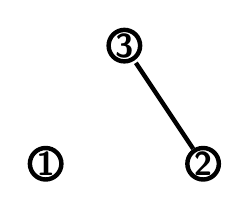
\begin{tikzpicture}[shorten >=1pt, auto, node distance=3cm, ultra thick,main node/.style={circle,draw,minimum size=.4cm,inner sep=0pt}]
\begin{scope}[every node/.style={font=\sffamily\large\bfseries}]
\node [main node](v1) at (0,0) {1};
\node [main node](v2) at (2,0) {2};
\node [main node](v3) at (1,1.5) {3};
\end{scope}
\path 
    (v2) edge (v3)
         ;
\end{tikzpicture}
Stan $VII\ \rightarrow\ S_{VII}$:\\
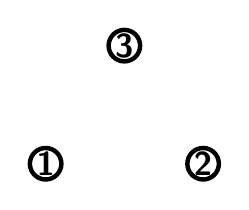
\begin{tikzpicture}[shorten >=1pt, auto, node distance=3cm, ultra thick,main node/.style={circle,draw,minimum size=.4cm,inner sep=0pt}]
\begin{scope}[every node/.style={font=\sffamily\large\bfseries}]
\node [main node](v1) at (0,0) {1};
\node [main node](v2) at (2,0) {2};
\node [main node](v3) at (1,1.5) {3};
\end{scope}
\end{tikzpicture}
\end{multicols}
\begin{itemize}
\item Jeżeli wypadł orzeł i wybrana krawędź należy do lasu $H$, to ją usuwamy.
\item Jeżeli wypadła reszka i wybrana krawędź nie należy do $H$, to dodajemy ją do $H$ (o ile nie domyka cyklu).
\item W przeciwnym wypadku nic nie robimy.
\end{itemize}
Budujemy łańcuch Markowa odpowiadający powyższemu algorytmowi, w którym stanami są wszystkie lasy rozpięte w $K_3$.
\begin{enumerate}[label=\alph*)]
\item Ile stanów ma ten łańcuch?

\textbf{Odpowiedź:} Łańcuch ma 7 stanów: $S=\{S_{I},S_{II},S_{III},S_{IV},S_{V},S_{VI},S_{VII},\}$
\item Proszę wybrać w $K_3$ drzewo rozpięte i podać wiersz macierzy przejścia łańcucha, odpowiadający temu stanowi.

\begin{align*}
&S_{I}\rightarrow S_{I}   & \frac{1}{2}*\frac{1}{3}+\frac{1}{2}=\frac{2}{3} &\text{ Orzeł i krawędź 2-3 albo Reszka}\\
&S_{I}\rightarrow S_{II}  & 0 &\text{ Nie da się w jednym kroku przejść z I do II}\\
&S_{I}\rightarrow S_{III} & 0 &\text{ Nie da się w jednym kroku przejść z I do III}\\
&S_{I}\rightarrow S_{IV}  & \frac{1}{2}*\frac{1}{3}=\frac{1}{6} &\text{ Orzeł i krawędź 1-3}\\
&S_{I}\rightarrow S_{V}   & \frac{1}{2}*\frac{1}{3}=\frac{1}{6} &\text{ Orzeł i krawędź 1-2}\\
&S_{I}\rightarrow S_{VI}  & 0 &\text{ Nie da się w jednym kroku przejść z I do VI}\\
&S_{I}\rightarrow S_{VII} & 0 &\text{ Nie da się w jednym kroku przejść z I do VII}
\end{align*}

$$\bar{P}(S_I)=\bbordermatrix{&S_{I}&S_{II}&S_{III}&S_{IV}&S_{V}&S_{VI}&S_{VII} \cr
S_I& \sfrac{2}{3} &0&0&\sfrac{1}{6}&\sfrac{1}{6}&0&0}$$
\item Czy łańcuch jest ergodyczny?

\textbf{Odpowiedź: }Gdybym napisał całą macierz, pewnie by wyszło, że z każdego stanu do każdego innego stanu bezpośrednio albo pośrednio mogę przejść.
\item Czy łańcuch jest odwracalny?

\textbf{Odpowiedź: }\textbf{CHYBA }Tak, gdyż zgodnie z definicja Odwracalności (\ref{def:OdwracalnoscLM2} na stronie \pageref{def:OdwracalnoscLM2}) gdybym zrobił całą macierz i wyliczył wektor własny, to by chyba wyszło.
\end{enumerate}

\paragraph{A5} Generujemy lasy rozpięte grafu $G$ następująco. Zaczynamy od dowolnego lasu rozpiętego, a w każdym kroku, Mając wygenerowany las $H$, wybieramy jednostajnie krawędź z $E(G)$ i z prawdopodobieństwem $\frac{1}{2}$ usuwamy ją z $H$ (Jeśli nie jest ona krawędzią $H$, to nic nie robimy), a z prawdopodobieństwem $\frac{1}{2}$ dodajemy ją do $H$ (o ile nie domyka cyklu).
\begin{enumerate}[label=\alph*)]
\item Czy łańcuch jest odwracalny?

\textbf{Odpowiedź: }Tak, Dowód przedstawiony w zadaniu \ref{par:10-A2} (strona \pageref{par:10-A2})
\item Czy jest ergodyczny?

\textbf{Odpowiedź: }Tak, Dowód przedstawiony w zadaniu \ref{par:10-A2} (strona \pageref{par:10-A2})
\item Czy możemy stwierdzić, że po wielu krokach każdy las rozpięty będzie w przybliżeniu jednakowo prawdopodobny?

\textbf{Odpowiedź: }Tak, Dowód przedstawiony w zadaniu \ref{par:10-A2} (strona \pageref{par:10-A2})
\end{enumerate}

\subsection{Zadania domowe B}
\paragraph{B1} Tasujemy talię $n$ ($n \geq 2$) kart w taki sposób: zaczynamy od dowolnego stosu, wybieramy losowo (z jednakowym prawdopodobieństwem) jedną z $n$ kart i kładziemy ją na wierzch.
\begin{enumerate}[label=\alph*)]
\item Sprawdź, że rozkład jednostajny jest rozkładem stacjonarnym tego łańcucha.
\item Uzasadnij, że łańcuch jest nieokresowy i nieprzywiedlny.
\item Czy po wielu krokach uzyskamy każde potasowanie z prawdopodobieństwem w przybliżeniu jednakowym?
\end{enumerate}

\paragraph{B2} Zaproponuj algorytm oparty na łańcuchu Markowa o $2^k$ stanach, który po wielu krokach wygeneruje każdy wierzchołek $k$-kostki z prawdopodobieństwem w przybliżeniu jednakowym. Zakładamy, że $k$ jest duże i stworzenie listy wszystkich $2^k$ wierzchołków $k$-kostki jest nieekonomiczne.

\paragraph{B3} Opisz zwięźle ideę algorytmu, generującego losowe skojarzenia w grafie (w tym zbiór pusty), w taki sposób, by każde ze skojarzeń $M$ wylosowane zostało z prawdopodobieństwem
\begin{enumerate}[label=\alph*)]
\item prawie jednakowym.
\item  bliskim
$$\frac{5^{|M|}}{\sum _S 5^{|S|}}$$
gdzie $|M|$ jest liczbą krawędzi w skojarzeniu $M$, a suma w mianowniku przebiega wszystkie skojarzenia
grafu (i zbiór pusty).
\item bliskim 
$$\frac{1}{3^{|M|*\sum _S\left(\sfrac{1}{3}\right)^{|S|}}}$$
gdzie $|M|$ jest liczbą krawędzi w skojarzeniu $M$, a suma w mianowniku przebiega wszystkie skojarzenia
grafu (i zbiór pusty). 
\end{enumerate}
Najważniejszą częścią tego zadania jest uzasadnienie poprawności algorytmu.

\paragraph{B4} Graf $G$ na $4$ wierzchołkach, będący cyklem z przekątną. Mamy też 3 kolory (czyli mniej niż $\Delta + 2$). Generujemy wszystkie właściwe kolorowania wierzchołków grafu $G$ następująco:
\begin{itemize}
\item Mając kolorowanie właściwe, wylosuj jeden z czterech wierzchołków $v$, każdy z jednakowym prawdopodobieństwem i wylosuj jeden z trzech kolorów $i$, każdy z jednakowym prawdopodobieństwem.
\item Jeśli po przemalowaniu wierzchołka $v$ na kolor $i$ kolorowanie pozostaje właściwe, przemaluj $v$ na kolor $i$.
\item W przeciwnym przypadku pozostaw kolorowanie bez zmian.
\end{itemize}
\begin{enumerate}[label=\alph*)]
\item Narysuj graf skierowany, obrazujący łańcuch Markowa odpowiadający podanemu algorytmowi. Zbiorem
stanów powinny być wszystkie właściwe kolorowania grafu $G$.
\item Czy po bardzo dużej liczbie kroków każde właściwe kolorowanie będzie w przybliżeniu jednakowo prawdopodobne, niezależnie jaki był stan początkowy?
\end{enumerate}


\paragraph{B5} Mamy $3$ kolory i graf $G = C_4$, czyli będący cyklem o $4$ wierzchołkach. Generujemy wszystkie właściwe kolorowania wierzchołków grafu $G$ następująco:
\begin{itemize}
\item Mając kolorowanie właściwe, wylosuj jeden z wierzchołków $v$, każdy z jednakowym prawdopodobieństwem i wylosuj jeden z kolorów $i$, każdy z jednakowym prawdopodobieństwem.
\item Jeśli po przemalowaniu wierzchołka $v$ na kolor $i$ kolorowanie pozostaje właściwe, przemaluj $v$ na kolor $i$.
\item W przeciwnym przypadku pozostaw kolorowanie bez zmian.
\end{itemize}
\begin{enumerate}[label=\alph*)]
\item Ile stanów ma łańcuch Markowa odpowiadający podanemu algorytmowi? Zbiorem stanów powinny być
wszystkie właściwe kolorowania grafu $G$.
\item Wyznacz pierwszy wiersz macierzy przejścia tego łańcucha (stan numer jeden wybierz samodzielnie).
\item Czy po bardzo dużej liczbie kroków każde właściwe kolorowanie będzie w przybliżeniu jednakowo prawdopodobne, niezależnie jaki był stan początkowy?
\item Jeśli w poprzednim podpunkcie zapomniałeś sprawdzić, czy łańcuch jest ergodyczny, zrób to teraz.
\end{enumerate}


\paragraph{B6} Mamy $n$ przedmiotów, o objętościach odpowiednio $v_1, . . . , v_n$. Mamy też plecak o pojemności $b$. Plecak możemy zapakować wybierając dowolnie zestaw przedmiotów (w tym zestaw pusty), o ile suma ich objętości nie przekracza pojemności plecaka. Zaproponuj algorytm oparty na łańcuchu Markowa, który po wielu krokach wybierze zestaw przedmiotów możliwy do zapakowania w taki sposób, by przybliżone prawdopodobieństwo wylosowania zestawu było funkcją rosnącą liczby przedmiotów w zestawie. Najważniejszą częścią zadania jest uzasadnienie poprawności algorytmu.

\paragraph{B7 *} Na wykładzie został tak zdefiniowany łańcuch Markowa na rodzinie wszystkich zbiorów niezależnych grafu, że współrzędne rozkładu stacjonarnego były proporcjonalne wykładniczo do rozmiaru zbioru. Skonstruuj łańcuch Markowa na rodzinie wszystkich zbiorów niezależnych grafu w taki sposób, aby współrzędne rozkładu stacjonarnego były proporcjonalne liniowo do rozmiaru zbioru.

\subsection{Zadania}
\paragraph{Zad.1} Wygeneruj za pomocą łańcucha Markowa o $2^n$ stanach wszystkie podzbiory zbioru $n$– elementowego tak, aby
\begin{enumerate}[label=\alph*)]
\item w rozkładzie stacjonarnym dla tego procesu wszystkie podzbiory były jednakowo prawdopodobne.
\item po wielu krokach otrzymać każdy podzbiór z prawdopodobieństwem w przybliżeniu jednakowym.
\item przybliżone prawdopodobieństwo wylosowania zbioru było funkcją rosnącą jego rozmiaru.
Zakładamy, że $n$ jest duże i stworzenie listy wszystkich $2^n$ podzbiorów jest nieekonomiczne.
\end{enumerate}

\paragraph{Zad.2} Lisek Chytrusek zaproponował poniższy algorytm (oparty na łańcuchu Markowa) do dobrego potasowania 52 kart. Celem liska było stworzyć algorytm, który po wielu krokach (np. 100tys) wygeneruje każde potasowanie z prawdopodobieństwem w przybliżeniu jednakowym. Algorytm liska: Zaczynam od dowolnego potasowania. W każdym kroku wybieram losowo kolejno dwie, niekoniecznie różne, karty (każdą losuję jednostajnie) i zamieniam miejscami. Sprawdź poprawność algorytmu.

\paragraph{Zad.3} Oto znany problem plecakowy. Mamy $n$ przedmiotów, o objętościach odpowiednio $v_1, . . . , v_n$. Mamy też plecak o pojemności $b$. Plecak możemy zapakować wybierając dowolnie zestaw przedmiotów (w tym zestaw pusty), o ile suma ich objętości nie przekracza pojemności plecaka. Zaproponuj algorytm oparty na łańcuchu Markowa, który po wielu krokach wybierze zestaw przedmiotów możliwy do zapakowania w sposób w przybliżeniu jednostajny (tzn. każdy zestaw będzie z grubsza jednakowo prawdopodobny).

\section[Wykład 10: 18-V-2017 - Temat: Teoria kodów]{Temat: Teoria kodów}
\subsection{Podstawowe definicje}
\begin{description}
\item[$Q$] alfabet $$Q=\{0,1,2,\dots ,q-1\}$$
$|Q|=q$ $\rightarrow$ liczba elementów alfabetu.\\
Na przykład:\\
$Q=\{0,1\}\rightarrow$ kody binarne, gdzie $|Q|=q=2$
\item[$n$] długość słowa
\end{description}
inne przykłady kodów:
\begin{itemize}
\item Kod ASCII $0-127\rightarrow 2^7$ gdzie ostatni bit to bit parzystości (mowa o historii)
\item PESEL, przykłady:
\begin{itemize}
\item[] $11304900014\rightarrow$ zły kod PESEL - dzień miesiąca 49? 
\item[] $11300900014\rightarrow$ niepoprawny kod PESEL
\item[] $11304900014\rightarrow$ kom mogący być kodem PESEL
\end{itemize}
\end{itemize}

\subsection{Teoria kodów:}
\begin{observation*}
Istnieje $q^n$ różnych słów długości $n$ nad alfabetem $Q$, $|Q|=q$.
\end{observation*}
\begin{definition}[Kod]
Kodem $C$ o długości $n$ nad alfabetem $Q$ nazywamy dowolny podzbiór o długości $n$ którego literami są elementy alfabetu $Q$ co zapisujemy: $$C\subseteq Q^n$$
Przykładowo słowo $\bar{x}=010111$ będziemy traktować jako wektor (kolumnowy) o argumentach $010111$, czyli: $$\bar{x}=\begin{bmatrix}
0\\1\\0\\1\\1\\1
\end{bmatrix}$$
\end{definition}
\begin{definition}[Odległość Hamminga]
W teorii kodów wyznaczamy \textbf{odległość Hamminga} to znaczy: $$d(\bar{x},\bar{y})=|\{j:x_i\neq y_i\}|$$
\begin{multicols}{2}
$$\bar{x}=0,1,2,5,7,1$$
$$\bar{y}=0,1,1,5,6,1$$
$$\bar{z}=7,1,2,5,7,1$$
\vfill\null
\columnbreak
$$d(\bar{x},\bar{y})=2$$
$$d(\bar{x},\bar{z})=1$$
\end{multicols}
\end{definition}

\begin{definition}[Rozstęp kodu]
\textbf{Rozstępem kodu} $C$ nazywamy najmniejszą odległość pomiędzy wyrazami tego kodu: $$r(C)=\min _{\begin{matrix}
\bar{x},\bar{y}\in C\\
\bar{x}\neq \bar{y}
\end{matrix}}d(\bar{x},\bar{y})$$
\end{definition}
\begin{observation*}
Jeśli chcemy by kod $C$ był odporny na zakłócenia komunikacji powudujące co najwyżej $r$ błędów to: $$r(C)=2R+1$$
\end{observation*}
\begin{problem*}
Oszacować liczbę wyrazów w kodzie $C$ o długości $n$ i rozstępie $r(C)=2R+1$
\end{problem*}
\subsection{Oszacowanie objętościowe}
\begin{itemize}
\item Weźmy $\bar{x}$
\item Ile jest wyrazów $\bar{y}$ takich, że $d(\bar{x},\bar{y})\leq r$?\\
Ile jest wyrazów w kuli o środku w $\bar{x}$ i promieniu $r$?\footnote{\#Shame: $\binom{n}{k}=\frac{n!}{k!(n-k)!}$}
\begin{align*}
&\text{Dane: }n\ \bar{x}=00\dots 0,\ Q=\{0,1,\dots ,q-1\}\\
&|\{\bar{y}:d(\bar{x},\bar{y})=0\}|=1\\
&|\{\bar{y}:d(\bar{x},\bar{y})=1\}|=n(q-1)\\
&|\{\bar{y}:d(\bar{x},\bar{y})=2\}|=\binom{n}{2}(q-1)(q-1)\\
&|\{\bar{y}:d(\bar{x},\bar{y})=i\}|=\binom{n}{i}(q-1)^i\\
&\sum _{i=0}^R\binom{n}{i}(q-1)^i\\
&|C|\sum _{i=0}^R\binom{n}{i}(q-1)^i\leq q^n\\
&|C|\leq  q^n\left(\sum _{i=0}^R\binom{n}{i}(q-1)^i\right)^{-1}
\end{align*}
\end{itemize}
\begin{definition}[Kod doskonały]
Kod $C$ o długości $n$ i odstępie $r(C)=2R+1$ nazywamy \textbf{doskonałym} gdy: $$|C|\sum _{i=0}^R\binom{n}{i}(q-1)^i= q^n$$
\end{definition}
\begin{example*}
4 kod ternarny $C_4(9)$ składający się z 9 słów: $$0000,0111,0222,1021,2012,1102,2201,2120,1210$$ jest kodem doskonałym o rozstępie 3:
\begin{align*}
&n=4,\ q=3,\ r=1,\ |C|=9\\
&9*\sum_{i=0}^R(q-1)^i=9*\left(1*2^0+4*2^1\right)=9*9=3^4
\end{align*}
\end{example*}

\subsection{Kody liniowe}
\begin{definition}[Kody Liniowe]
Niech $F_q$ będzie ciałem o $q$ elementach.\\ Takie ciało istnieje wtedy i tylko wtedy, gdy $q$ jest potęgą liczby pierwszej $$q=p^n$$ $p\rightarrow$ liczba pierwsza.\\ Na naszych zajęciach zawsze będziemy zakładać, że $q$ jest liczbą pierwszą.
\begin{align*}
&q\rightarrow\text{Liczba pierwsza}\\
&F_q=\{0,1,2,\dots ,q-1\}\\
&\text{Operacje: }\\
&&+ (\mod q)\\
&&* (\mod q)
\end{align*}
\end{definition}
\begin{example*}
Dla $F_7$ załóżmy, że mamy równanie:
\begin{align*}
&6x=2\\
&6x\equiv  2 (\mod 7)\\
&x \equiv 5
\end{align*}
\end{example*}

Jeśli mamy kilka wektorów $\bar{x}_1,\bar{x}_2,\dots ,\bar{x}_n\in Q^n=F_q^n$
$$\alpha _1 \bbordermatrix{&\bar{x}_1\cr
&\vdots\cr &\vdots\cr &\vdots}+\alpha _2 \bbordermatrix{&\bar{x}_2\cr
&\vdots\cr &\vdots\cr &\vdots}+\dots +\alpha _n \bbordermatrix{&\bar{x}_n\cr
&\vdots\cr &\vdots\cr &\vdots}=\bbordermatrix{&\bar{y}\cr
&\vdots\cr &\vdots\cr &\vdots}$$

\begin{definition}[ n,k kod]
Kodem $[n,k]$ będziemy nazywali dowolną podprzestrzeń liniową $C$ wymiaru $k$ w $F_q^n=Q^n$.\\$[n,k]$ kod $C$ nazywamy $[n,k,d]$ kodem jeśli $r(C)=d$
\end{definition}

\begin{definition}[Wektor bazowy]
Niech $\bar{x}_1,\bar{x}_2,\dots ,\bar{x}_k$ będą wektorami bazowymi $C$, to znaczy każdy element $\bar{y}\in C$ da się przedstawić w sposób jednoznaczny jako kombinację $\bar{x}_1,\bar{x}_2,\dots ,\bar{x}_k$ to znaczy istnieją $\alpha _1,\alpha _2,\dots ,\alpha _k \in Q$ takie, że:
$$\bar{y}=\alpha _1\bar{x}_1+\alpha _2\bar{x}_2+\dots +\alpha _k\bar{x}_k$$
\textbf{Pytanie:} ile elementów ma $[n,k]$ kod?\\
\textbf{Odpowiedź:} $$\underbrace{q*q*\dots *q}_k=q^k$$
\end{definition}
\begin{example*}[Przykład z kodu termanego]
9 słów, $Q=3$, $9=3^2$ $[4,2]$, $|C|=9$
$$\bar{y}=\alpha _1\begin{bmatrix}
0\\1\\1\\1
\end{bmatrix}+\alpha _2\begin{bmatrix}
1\\0\\2\\1
\end{bmatrix}\Leftrightarrow \begin{bmatrix}
2\\1\\2\\0
\end{bmatrix}=1\begin{bmatrix}
0\\1\\1\\1
\end{bmatrix}+2\begin{bmatrix}
1\\0\\2\\1
\end{bmatrix}$$
\end{example*}

\begin{definition}[Macierz generująca]\textbf{Macierzą generującą} $G$ $[n,k]$ kodu $C$ generowanego przez bazę $\bar{x}_1,\bar{x}_2,\dots ,\bar{x}_k$ nazywamy macierz, której wierszami są wektory: $\bar{x}_1^T,\bar{x}_2^T,\dots ,\bar{x}_k^T$

Dla przykładu powyżej:
$$G=\begin{bmatrix}
0&1&1&1\\
1&0&2&1
\end{bmatrix},\ G=\begin{bmatrix}
0&2&2&2\\
1&2&1&0
\end{bmatrix}$$
Zauważmy, że $$C=\{\alpha ^Y*G:\alpha ^T\in G^k\}$$
Dalej ten sam przykład:
$$[ 1, 2 ] \begin{bmatrix}
0&1&1&1\\
1&0&2&1
\end{bmatrix}=\begin{bmatrix}
2&1&2&0
\end{bmatrix}=1*\begin{bmatrix}
0&1&1&1
\end{bmatrix}+2\begin{bmatrix}
0&1&1&1
\end{bmatrix}$$
\end{definition}



\begin{definition}[Macierz parzystości]
\textbf{Macierzą parzystości} $H$ $[n,k]$ kodu $C$ jest macierz o rozmiarze $(n-k)\times n$ o rzędzie $n-k$ taka, że $$GH^T=O$$ gdzie $O$ oznacza macierz zerową. 
\end{definition}
\begin{fact*}
Słowo $\bar{y}\in C$ wtedy i tylko wtedy, gdy $K\bar{y}=0$
\end{fact*}

\begin{definition}[Ortogonalność]
W przestrzeni liniowej z iloczynem skalarnym $<\ >$ wektory $u,v\in V$ są \textbf{ortogonalne} (lub prostopadłe) gdy $<u,v>=0$. Piszemy wtedy $u\bot v$.
\end{definition}

\begin{definition}[Układ ortogonalny, układ ortonormalny]
Mówimy, że układ wektorów $(v_i)_{i\in I}$ z przestrzeni $V$ jest \textbf{układem ortogonalnym} gdy $<v_j, v_k> = 0$ dla $j\neq k$ . \textbf{Układ} jest \textbf{ortonormalny} gdy jest ortogonalny oraz $<v_j
, v_j> = 1$ dla $j\in I$.
\end{definition}


\section{Ćwiczenia 11: 18-V-2017}
\subsection{Zadania domowe A}
\paragraph{A1} Dany jest kod $C$ nad alfabetem $Q$, składający się ze słów:
$$(0, 1, 0, 1), (1, 0, 1, 1), (0, 0, 0, 0), (1, 1, 1, 0)$$
\begin{enumerate}[label=\alph*)]
\item Dla $y = (1, 0, 0, 1)$ wyznacz jego odległość do najbliższego słowa kodu, czyli $\min _{x \in C} d(y, x)$. Czy tu istotne jest, nad jakim alfabetem $Q$ określony jest kod $C$?

Kod $C: (0, 1, 0, 1), (1, 0, 1, 1), (0, 0, 0, 0), (1, 1, 1, 0)$ , Alfabet (zapewne) $Q=\{0,1\} $
\begin{align*}
&x_1,x_2,x_3x,_4\in C\\
x_1: &(0, 1, 0, 1) & d(y,x_1)=2\\
x_2: &(1, 0, 1, 1) & d(y,x_2)=1\\
x_3: &(0, 0, 0, 0) & d(y,x_3)=2\\
x_4: &(1, 1, 1, 0) & d(y,x_4)=3\\
&\min _{x\in C}(y,x)=1
\end{align*}
\item Znajdź rozstęp kodu $C$. Czy dla określenia rozstępu istotne jest, jaki jest alfabet $Q$?

\begin{align*}
&d(x_1,x_2)=3&d(x_2,x_3)=3&d(x_3,x_4)=3\\
&d(x_1,x_3)=2&d(x_2,x_4)=2\\
&d(x_1,x_4)=3\\
&\min _{\begin{matrix}
x,y\in C\\
x\neq y
\end{matrix}} d(x,y)=2
\end{align*}
Do określenia rozstępu \textbf{nie jest} istotna wiedza na temat alfabet $Q$, ważna jest odległość pomiędzy wyrazami tego kodu.
\item Załóżmy, że $C$ jest kodem binarnym, tzn. $Q = \{0, 1\}$. Wypisz wszystkie elementy kuli Hamminga w przestrzeni $Q^4$, o środku w wybranym przez siebie słowie kodu i o promieniu 2. Czy dla liczby tych elementów istotne jest, nad jakim alfabetem $Q$ określony jest kod $C$?

\begin{align*}
&Q^4,\ Q=\{0,1\}\\
&\text{Środek: } (0,0,0,0)\\
&\text{Elementy: } (0,0,0,0), (0,0,0,1), (0,0,1,0), (0,0,1,1), (0,1,0,0), (0,1,0,1), (0,1,1,0), (1,0,0,0), (1,0,0,1),\\
&(1,0,1,0), (1,1,0,0), (1,0,0,1)\\
&\text{Liczba: } |\{\bar{y}:d(\bar{x},\bar{y})=2\}|=\binom{n}{2}(q-1)(q-1)\\
&\text{Wzór dla promienia }i:\ |\{\bar{y}:d(\bar{x},\bar{y})=i\}|=\binom{n}{i}(q-1)^i
\end{align*}
Tak jest istotne zgodnie z wyżej wymienionym wzorem na liczbę wyrazów w kuli o środku w $\bar{x}$ i promieniu 2 jak i również promienia $i$.
\end{enumerate}


\paragraph{A2} Niech $Q = \{0, 1, 2\}$ i $y = (0, 1, 2, 1, 0)$.
\begin{enumerate}[label=\alph*)]
\item Podaj przykład kodu $C \subseteq Q^5$ (wypisując wszystkie jego słowa), który ma rozstęp 2, a dla słowa $y$ istnieje dokładnie jedno słowo kodu w odległości 1 od $y$.

\begin{align*}
&y = (0, 1, 2, 1, 0)\\
&C=(11210)(01010)(00210)(01200)(01212)
\end{align*}
\item Wypisz wszystkie elementy kuli Hamminga w przestrzeni $Q^5$, o środku $y$ i promieniu 1.

\item Ile jest słów przestrzeni $Q^5$ w odległości 2 od $y$?
$$\sum _{i=0}^R\binom{n}{i}(q-1)=\binom{5}{0}(3-1)^0+\binom{5}{1}(3-1)^1+\binom{5}{2}(3-1)^2$$
\end{enumerate}

\paragraph{A3} Załóżmy, że $Q$ jest alfabetem 4-elementowym. Ile elementów ma kula Hamminga o promieniu 3 w przestrzeni $Q^6$?

\begin{align*}
&Q=(0,1,2,3)\\
&R=3,\ Q^6,\ n=6\\
&\sum _{i=0}^3\binom{6}{i}(q-1)^i
\end{align*}

\paragraph{A4} Wyznacz rozstęp podanego kodu ternarnego, czyli nad alfabetem $Q = \{0, 1, 2\}$.
$$C = \{(0, 0, 0, 0),(2, 1, 0, 1),(2, 2, 1, 0),(1, 0, 1, 1),(1, 1, 2, 0),(1, 2, 0, 2),(2, 0, 2, 2),(0, 1, 1, 2),(0, 2, 2, 1)\}$$

\begin{align*}
&Q=\{0,1,2\}\\
&r(C)=\min d(\bar{x}, \bar{y})\\
&r(C)=3
\end{align*}
przeanalizowałem że tak jest.

\paragraph{A5} Załóżmy, że dla kodów $C$ i $C'$ zachodzi $C\subseteq C'$. Jaka jest relacja między ich rozstępami $r(C)$ i $r(C')$ ?

\begin{figure}[H]
\centering
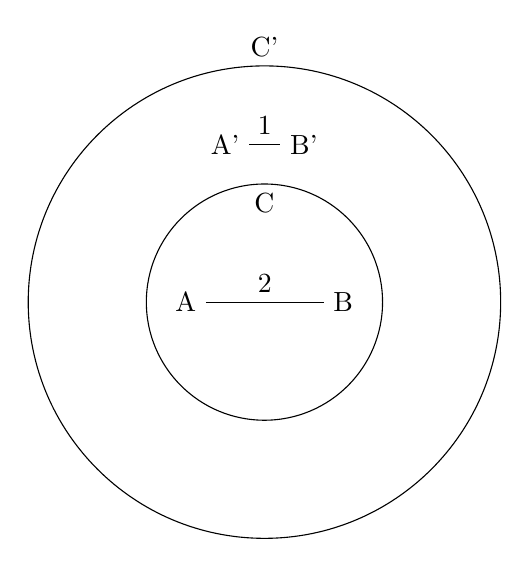
\begin{tikzpicture}
\draw  (0,0) node (v1) {} ellipse (3 and 3);
\draw  (v1) ellipse (1.5 and 1.5);
\node (v2) at (-1,0) {A};
\node (v3) at (1,0) {B};
\draw  (v2) edge node [above] {2} (v3);
\node (v4) at (-0.5,2) {A'};
\node (v5) at (0.5,2) {B'};
\node[below] (c1) at (0,1.5) {C};
\node[above] (c2) at (0,3) {C'};
\draw  (v4) edge node [above] {1} (v5);
\end{tikzpicture}
\end{figure}
$$r(C)\geq r(C')$$
Zgodnie z definicją rozstępu - szukamy jak najmniejszej odległości między wyrazami kodu. Wiemy, że $C\subseteq C'$ czyli, jeżeli najmniejszy rozstęp znajduje się w $C$ to jest on również e $C'$ jednakże, przez to, że $C'$ jest ,,większe'' to istnieje prawdopodobieństwo, że odległość między dwoma wyrazami ciągu w $C'$ będzie ,,mniejsza''.
\paragraph{A6} Korzystając z definicji doskonałości, uzasadnij, że
\begin{enumerate}[label=\alph*)]
\item kod $C = \{(0, 0, 0, 0),(1, 1, 1, 1)\} \subseteq \{0, 1\}^4$ nie jest doskonały.


Kod $C$ o długości $i$ i rozstępie $r(C)=2R+1$ nazywamy doskonałym, gdy:
$$|C|\sum_{i=0}^{\floor{\sfrac{r(C)}{2}}}\binom{n}{i}(q-1)^i=q^n$$
Dla: $|C|=2$, $n=4$ Kod $C$ o roztępie $r(C)=2R+1$ nazywany doskonałym, gdy dla każdego słowa alfabetu $x\in Q$ istnieje dokładnie jedno słowo kodu $y\in C$ takie, że $d(x,y)\leq R$.

$C$ jest \textbf{niedoskonały}, ponieważ kod $0011$ ma najbliższe kody: $0000$ i $1111$ a powinien mieć tylko 1 w odległości $R=\floor{\frac{r(C)}{2}}=2$
\begin{align*}
&|C|\sum_{i=0}^{\floor{\sfrac{r(C)}{2}}}\binom{n}{i}(q-1)^i = |C|\sum_{i=0}^{2}\binom{4}{i}(2-1)^i=2*(1+4+6)=22\\
&q^n=2^4=16\\
&22\neq 16
\end{align*}
\item kod $C = \{(0, 0, 0),(1, 1, 1)\} \subseteq \{0, 1\}^3$ jest doskonały. 

$n=3$, $|Q|=q=2$, $|C|=2$ $r(C)=3$ $R=\floor{\frac{r(C)}{2}}=1$
\begin{align*}
&2*\sum _{i=0}^1\binom{3}{1}(1=2(1+3=8\\
&q^n=2^3=8\\
&8=8
\end{align*}
\end{enumerate}
Nie można w tym zadaniu korzystać z podanego na wykładzie twierdzenia o kodach doskonałych.

\paragraph{A7} Dany jest kod ternarny $C \subseteq \{0, 1, 2\}^5$:
$$C = \{(0, 0, 0, 0, 0),(1, 2, 1, 0, 0),(2, 1, 2, 0, 0),(0, 1, 1, 2, 1),(0, 2, 2, 1, 2),(2, 0, 1, 1, 2),(1, 0, 2, 2, 1),(2, 2, 0, 2, 1),(1, 1, 0, 1, 2)\}$$
\begin{enumerate}[label=\alph*)]
\item Jaki jest jego rozstęp?

$r(C)=3$ (trzeba znaleźć)
\item Znajdź przykładowy $y \in \{0, 1, 2\}^5$, którego odległość do najbliższego mu słowa kodu $C$ wynosi 2.

$y=(11002)$
\item Czy $C$ jest kodem doskonałym?

\begin{align*}
&R=\floor{\frac{r(C)}{2}},\ n =5,\ q=3,\ |C|=9\\
&|C|\sum ^R_{i=0}\binom{n}{i}(3-1)^i=99\\
&q^n=3^5=243\\
&99=neq 243
\end{align*}
Kod nie jest doskonały.
\end{enumerate}

\paragraph{A8} Rozważmy taki kod ternarny $C \subseteq \{0, 1, 2\}^{10}$ : $C = \{(x, x, x, x, x, y, y, y, y, y): x, y \in {0, 1, 2}\}$.
\begin{enumerate}[label=\alph*)]
\item Ile słów należy do kodu $C$ i jaki jest jego rozstęp?

Do kodu $C$ należy $9$ ($X$ wybieramy na 3 sposoby i $y$ również wybieramy na 3 sposoby - nie jest napisane, że są różne!) więc $r(C)=5$
\item Czy $C$ jest kodem doskonałym ?

$$9*\left(\sum _{i=0}^R \binom{n}{i}(q-1)^i\right)$$
\end{enumerate}

\paragraph{A9} Oceń poprawność poniższych zdań. Odpowiedź należy poprzeć, jak zwykle, albo uzasadnieniem ogólnym, albo przykładem, albo kontrprzykładem. poprawność przykładu/kontrprzykładu też należy uzasadnić.
\begin{enumerate}[label=\alph*)]
\item Jeśli $|C| > 2$ i kod $C \subseteq Q^n$ ma rozstęp $k$, to każde dwa różne słowa tego kodu są w odległości dokładnie $k$.

\textbf{NIE} definicja rozstępu: $r(C)=\min _{\begin{matrix}
\bar{x}\bar{y}\in C\\
\bar{x}\neq\bar{y}
\end{matrix}}d(\bar{x}\bar{y})$ więc poszczególna odległość może być większa na przykład:
\begin{align*}
&Q^3,\ \ Q=\{0,1\}\\
&C=\{(0,0,0),(0,0,1),(1,1,1)\}\\
&r(C)=1\text{, ale }d(\bar{c}_1,\bar{c}_3)=3
\end{align*}
\item Jeśli $|C| > 2$ i kod $C \subseteq Q^n$ ma rozstęp $k$, to istnieją dwa różne słowa tego kodu są w odległości dokładnie $k$.

\textbf{TAK} wynika z definicji rozstępu:
$$r(C)=\min _{\begin{matrix}
\bar{x}\bar{y}\in C\\
\bar{x}\neq\bar{y}
\end{matrix}}d(\bar{x}\bar{y})$$
\item Jeśli $|C| > 2$ i kod $C \subseteq Q^n$ ma rozstęp $k$, to każde dwa różne słowa tego kodu są w odległości przynajmniej $k$.

\textbf{TAK} wynika z definicji rozstępu:
$$r(C)=\min _{\begin{matrix}
\bar{x}\bar{y}\in C\\
\bar{x}\neq\bar{y}
\end{matrix}}d(\bar{x}\bar{y})$$
\item Istnieje kod binarny o rozstępie 4.

\textbf{TAK} na przykład:
\begin{align}
&Q=\{0,1\}\ n=4,\ q=2\\
C=\{(0000),(1111)\}\ |C|=2
\end{align}
\item Istnieje kod ternarny długości 5, o rozstępie 4, złożony z 4 słów.

\textbf{TAK} 
$$C=\{(11110),(00000),(02222),(20121)\}$$
\item Istnieje binarny kod doskonały długości 2, złożony z mniej niż 4 słów.

\textbf{NIE} możliwe słowa kodu binarnego: $C=\{(00),(01),(10),(11)\}$ i zgodnie z definicją kodu doskonałego 
\item Istnieje kod ternarny doskonały, o rozstępie 3, złożony z 6 słów.

\textbf{NIE}
\begin{align*}
&|C|\sum _{i=0}^R\binom{n}{i}(q-1)^i= q^n\\
&6\sum_{i=0}^1\binom{n}{i}(3-1)^i=3^n\\
&6(6)1+\binom{n}{1}(2)^n=3^n\\
&6\left(1+2\binom{n}{1}\right)=3^n\\
&6+12\frac{n!}{(n-1)!}=3^n\\
&6+12n=3^n
\end{align*}
Potęgami liczby 3 są liczby nieparzyste, podczas gdy wyrażenie $6+12n$ zawsze w wyniku będzie dawało liczbę parzystą $\rightarrow$ SPRZECZNOŚĆ!
\item Istnieje kod ternarny doskonały, złożony z 6 słów.

\textbf{NIE}
\begin{align*}
&|Q|=q=3\ |C|=6\\
&
\end{align*}
\item Istnieje kod (niekoniecznie binarny, niekoniecznie ternarny) złożony z 64 słów długości 5, który ma rozstęp 3.

\textbf{TAK} \begin{align*}
& |C|=64,\ \ n=5,\ \ r(C)=3\\
& 64 \sum_{i=0}^i \binom{5}{1}(q-1)^1=q^5\\
& 64(1+5(q-1))=q^5\\
& 320q-256=q^5\\
& q = 4
\end{align*}
Tak istnieje, dla $q=4$
\item Jeżeli kod $C \subseteq Q^n$ ma rozstęp 5, to w $Q^n$ nie istnieje słowo będące w odległości 2 od dwóch różnych słów kodu $C$.

\textbf{NIE} 
Warunek trójkąta
\begin{figure}[H]
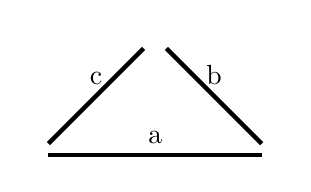
\begin{tikzpicture}[ultra thick]%,mian node/.style={draw,shape=circle,fill=blue}]
\node (v1) at (0,0) {};
\node (v2) at (3,0) {};
\node (v3) at (1.5,1.5) {};
\draw  (v1) edge node[above] {a} (v2);
\draw  (v2) edge node[above] {b} (v3);
\draw  (v3) edge node[above] {c} (v1);
\end{tikzpicture}
\end{figure}
zgodnie z prawem trójkąta $b+c>a$ a przypadku danych z zadania $a=5$ i $b=c=2$ no nie bangla...
\item Jeżeli rozstęp $r(C)$ kodu $C$ jest liczbą nieparzystą, to nie istnieje słowo będące w odległości co najwyżej $\sfrac{r(C)}{2}$ od dwóch różnych słów kodu $C$.

\textbf{NIE} zgodnie z definicją rozstępu $r(C)=\min _{\begin{matrix}
\bar{x}\bar{y}\in C\\
\bar{x}\neq\bar{y}
\end{matrix}}d(\bar{x}\bar{y})$ i domyślną definicją promienia.
\item Istnieje alfabet $Q$, liczba naturalna $n$ i kod $C \subseteq Q^n$ o nieparzystym rozstępie, dla którego $$|C|\sum ^{\floor{\sfrac{r(C){2}}}} _{j=0} \binom{b}{j}(|Q| - 1)^j > |Q|^n$$ $r(C)$ oznacza rozstęp kodu $C$.

\textbf{NIE} Oszacowanie objętościowe jest ograniczone ,,z lewej'':
$$|C|\sum ^{R} _{i=0} \binom{n}{j}(|Q| - 1)^j > |Q|^n$$
\end{enumerate}

\subsection{Zadania domowe B}
\paragraph{B1} W komunikacji z niektórymi sondami kosmicznymi stosowano następujące kodowanie korekcyjne: każdy bit źródłowej wiadomości przesyłany był pięciokrotnie, np. dla wiadomości 1011 wysyłane były cztery paczki: 11111 00000 11111 11111. Podczas transmisji możliwe były błędy: prawdopodobieństwo zmiany bitu wynosiło 0,05 dla każdego bitu. Podczas odczytu za poprawny bit wiadomości uznawało się ten, który w paczce bitów pojawiał się częściej. Na przykład paczka 10110 traktowana była jako bit 1, a paczka 10000 jako bit 0. Oblicz prawdopodobieństwo poprawnego odczytania wiadomości, która w wersji źródłowej składała się z 8 bitów. Jakie byłoby prawdopodobieństwo poprawnego odczytu, gdyby nie stosowano kodowania korekcyjnego, tzn. gdyby wysłano tylko 8 bitów wiadomości? Odpowiedzi podaj z dokładnością do 0,01.

\paragraph{B2} Niech $Q = \{0, 1, 2\}$ oraz $C = \{(2, 0, 1),(2, 1, 0)\}$.
\begin{enumerate}[label=\alph*)]
\item Wypisz wszystkie elementy kuli Hamminga w przestrzeni $Q^3$ o promieniu 2 i środku $(2, 0, 1)$.
\item Sprawdź, czy kod $C$ jest doskonały, Korzystając z definicji doskonałości.
\end{enumerate}

\paragraph{B3} Niech $Q = \{0, 1, 2, 3, 4\}$ oraz $C = \{(2, 0, 0, 1),(0, 1, 0, 0),(2, 1, 1, 2)\}$.
\begin{enumerate}[label=\alph*)]
\item Podaj przykład słowa, dla którego odległość od każdego ze słów kodu jest równa 3.
\item Czy kod $C$ jest doskonały?
\end{enumerate}


\paragraph{B4}
\begin{enumerate}[label=\alph*)]
\item Ile elementów liczy każda kula Hamminga o promieniu 3 w przestrzeni $\{0, 1, 2\}^{10}$?
\item Czy istnieje ternarny kod doskonały długości 5, o dokładnie 80 słowach?
\end{enumerate}

\paragraph{B5} W tym zadaniu przez $B(y, k)$ oznaczamy kule, (oczywiście Hamminga) o środku w $y$ i promieniu $k$. Załóżmy, że $C$ jest kodem binarnym długości 8, o rozstępie 3. Czy wynika z tego, że
\begin{enumerate}[label=\alph*)]
\item Dla każdych dwóch różnych słów $x, y \in C$ kule $B(x, 1)$ i $B(y, 1)$ są rozłączne?
\item Dla każdych dwóch różnych słów $x, y \in C$ kule $B(x, 2)$ i $B(y, 2)$ są nierozłączne?
\end{enumerate}

\paragraph{B6} Uzasadnij, że nie istnieje kod binarny $C$ długości 10 (niekoniecznie liniowy), dla którego $|C| = 32$ i rozstęp $C$ wynosi 5.

\paragraph{B7} Czy istnieje kod ternarny długości 7, o rozstępie 5, który ma dokładnie 27 słów?

\paragraph{B8} Opisz wszystkie binarne kody doskonałe o przynajmniej dwóch słowach i długości $n = 3, 4, 6, 8, 9$.

\paragraph{B9 *} Skonstruuj binarny kod doskonały o rozstępie 3 i długości 7.

\subsection{Zadania na ćwiczenia}
\paragraph{Zad.1} Opisz wszystkie binarne kody doskonałe o przynajmniej dwóch słowach i
\begin{enumerate}[label=\alph*)]
\item długości n = 9 i rozstępie 7.
\item długości n = 5.
\end{enumerate}


\paragraph{Zad.2} Lisek Chytrusek postanowił sprawdzić, czy istnieje binarny kod doskonały o długości 7 i rozstępie 3. Oceń poprawność podanego rozumowania liska. Przemykając pod oknami pewnego uniwersytetu, usłyszałem, że dla kodów doskonałych o rozstępie 3, długości $n$, nad alfabetem $Q$, zachodzi: $$|C| \sum ^{\floor{\sfrac{3}{2}}}_{i=0}\binom{n}{i}(|Q| - 1)^i = |Q|^n$$Podstawiając $|Q| = 2$ i $n = 7$, otrzymuje, $|C|* 8 = 27$. Zatem dla $|C| = 24$ to równanie jest spełnione. Czyli doskonały kod binarny o długości $7$ i rozstępie $3$ istnieje.

\paragraph{Zad.3} Wykaż, że każdy kod $C \subseteq Q^4$ nad alfabetem 5- elementowym, zawierający co najmniej 40 wyrazów ma rozstęp co najwyżej dwa.

\paragraph{Zad.4}
\begin{enumerate}[label=\alph*)]
\item Uzasadnij, że jeśli kod $C \subseteq \mathbb{Q}^n$ jest doskonały, to dla każdego $y\in \mathbb{Q}^n$ istnieje dokładnie jedno słowo kodu $C$, najbliższe słowu $y$, a w dodatku odległość $y$ do najbliższego słowa kodu nie przekracza $\floor{\sfrac{r(C)}{2}}$.
\item Uzasadnij, że dla dowolnego alfabetu $\mathbb{Q}$, jeżeli $x,y\in \mathbb{Q}^n$ i $d(x, y) = 2k$, to istnieje w $\mathbb{Q}^n$ słowo będące w odległości $k$ zarówno od $x$ jak i od $y$.
\item Czy może się zdarzyć, że dla pewnego kodu $C \subseteq \mathbb{Q}^n$ zachodzi
$$|C|\sum_{i=0}^{\floor{\sfrac{r(C)}{2}}}\binom{n}{i}(|Q|-1)^i>|Q|^n$$
$r(C)$ oznacza rozstęp kodu.
\item Czy może się zdarzyć, że dla pewnego kodu $C \subseteq \mathbb{Q}^n$ o parzystym rozstępie zachodzi
$$|C|\sum_{i=0}^{\floor{\sfrac{r(C)}{2}}}\binom{n}{i}(|Q|-1)^i=|Q|^n$$
\end{enumerate}

\paragraph{Zad.5} Sprawdzamy kawałki ostatnich dwóch zadań domowych.


%-------------------- WYKŁAD --------------------
\section[Wykład 11: 25-V-2017 - Temat: Teoria kodów II]{Temat: Teoria kodów II}
\subsection{Definicje}
$$Q=\{0,1,\dots,q-1\}=F_q$$
przyjmujemy, że $q$ to liczba pierwsza
$$c\subseteq Q^n$$
$$r(C)=\min_{\begin{matrix}
\bar{x},\bar{y}\in C\\
\bar{x}\neq\bar{y}
\end{matrix}}$$
Odległość Hamminga - czyli na ilu miejscach $\bar{x}$ różni się od $\bar{y}$

$[n,k]$-kod - podprzestrzeń liniowa $Q^n$ o wymiarze $k$

\begin{example*}[Przykład wykorzystywany w reszcie wykładu]
\begin{align*}
&C=\{(0,0,0,0),(0,1,1,1),(0,2,2,2),(1,0,2,1),(2,0,1,2),(1,1,0,2),(2,2,0,1),(1,2,1,0)\}\\
&Q=\mathbb{F}_3\\
&G=\begin{bmatrix}
0&0&2&1\\0&1&1&1
\end{bmatrix}\\
&G_2=\begin{bmatrix}
1&1&0&2\\2&0&1&2
\end{bmatrix}
\end{align*}
\end{example*}

\begin{definition}[Macierz parzystości]
Macierz sprawdzania parzystości (dalej nazywana \textbf{Macierzą parzystości}) $H$ to macierz, której wierszami jest $n-k$ niezależnych wektorów, z których każdy jest ortogonalny do każdego wiersza macierzy $G$.
\end{definition}
\begin{example*}
\begin{align*}
&H_1=\begin{bmatrix}
1&0&2&1\\0&1&1&1
\end{bmatrix}\\
&GH^T=[ {\Huge 0}]\\
&\begin{bmatrix}
1&0&2&1\\0&1&1&1
\end{bmatrix}\begin{bmatrix}
0&1\\1&0\\1&2\\1&1
\end{bmatrix}=\begin{bmatrix}
(0+0+2+1)\%3 & (1+0+4+1)\%3\\
(0+1+1+1)\%3 & (0+0+2+1)\%3 
\end{bmatrix}=\begin{bmatrix}
0&0\\
0&0
\end{bmatrix}
\end{align*}
Gdy macierz $G$ jest postaci (postać normalna):
$$G=\begin{bmatrix}
{\Huge I_k}& {\Huge P}
\end{bmatrix}$$
to
$$\begin{bmatrix}
{\Huge -P^T} & {\Huge I_{n-k}}
\end{bmatrix}$$ jest (jedną z) macierzy parzystości
\begin{align*}
&G_1=\begin{bmatrix}
1&0&2&1\\0&1&1&1
\end{bmatrix} & H_1=\begin{bmatrix}
1&2&1&0\\2&2&0&1
\end{bmatrix}\\
&\mathbb{F}_5\\
&G=\begin{bmatrix}
1&0&0&2&3\\
0&1&0&1&1\\
0&0&1&2&1
\end{bmatrix} & H=\begin{bmatrix}
3&4&3&1&0\\
2&4&4&0&1
\end{bmatrix}\\
&H=\left[{\huge -P^T\ I_{n-k}}\right]=\begin{bmatrix}
5-2 & 5-1 & 5-2 & 1 & 0\\
5-3 & 5-1 & 5-1 & 0 & 1
\end{bmatrix}\\
&G=\left[{\huge I_k\ P}\right]=\begin{bmatrix}
1 & 0 & 0 & 5-3 & 5-2\\
0 & 1 & 0 & 5-4 & 5-4\\
0 & 0 & 1 & 5-3 & 5-4
\end{bmatrix}
\end{align*}
\end{example*}

\begin{fact}
$$\bar{x}\in C\Leftrightarrow H\bar{x}=[0]$$
\end{fact}
\begin{example*}
Mając macierz parzystości $H=\begin{bmatrix}
1&2&1&0\\2&2&0&1
\end{bmatrix}$ czy wektor $\bar{x}=2120$ należy do $C$?

\begin{align*}
&H\bar{x}=[0]\\
&\begin{bmatrix}
1&2&1&0\\2&2&0&1
\end{bmatrix}\begin{bmatrix}
2\\1\\2\\0
\end{bmatrix}\Leftrightarrow \begin{bmatrix}
(2+2+2+0)\%3\\
(4+2+0+0)\%3
\end{bmatrix}=\begin{bmatrix}
0\\0
\end{bmatrix}
\end{align*}
\textbf{Odpowiedź: }tak wektor $\bar{x}$ należy do kodu $C$.

Czy wektor $\bar{y}=2200$ należy do $C$?
\begin{align*}
&H\bar{y}=[0]\\
&\begin{bmatrix}
1&2&1&0\\2&2&0&1
\end{bmatrix}\begin{bmatrix}
2\\2\\0\\0
\end{bmatrix}\Leftrightarrow \begin{bmatrix}
(2+4+0+0)\%3\\
(4+4+0+0)\%3
\end{bmatrix}=\begin{bmatrix}
0\\2
\end{bmatrix}
\end{align*}
\textbf{Odpowiedź: }NIENIU!
\end{example*}
\begin{problem}[Jak znaleźć wektor należący do $C$?]
\begin{align*}
H\bar{x}\neq \bar{0}& H\bar{x}=a\neq \bar{0}\\
&H\bar{y} =a\neq\bar{0}\\
&H(\bar{x}-\bar{y})=H\bar{x}-H\bar{y}=\bar{0}\\
&\bar{x}-\bar{y}\in C
\end{align*}
czyli trzeba znaleźć $\bar{y}$ taki, że $H\bar{y}=a$ i $\bar{y}$ ma jak najwięcej współrzędnych zerowych.
\end{problem}
\begin{align*}
\bar{x}=2200\\
\bar{y}=? &\bar{y}=0002\\
&\bar{x}-\bar{y}=2200-0002=2201
\end{align*}
\textbf{Pytanie:} Jak skonstruować kody doskonałe?
\begin{definition}[Kod Hamminga]
Kodem Hamminga nazywamy $[n, n-l, 3]$ kod nad ciałem $F_q$ taki, że: $$n=\frac{q^l-1}{q-1}$$

Macierz parzystości kodów Hamminga można wygenerować w prosty sposób: jako kolumny macierzy należy wziąć $n$ wektorów \textbf{parami niezależnych}.
\end{definition}
\begin{fact}
Kod Hamminga jest kodem doskonałym.
\end{fact}
\begin{example*}
\begin{align*}
q=5 & n=6 &l=2 \\
n=\frac{q^l-1}{q-1} & \rightarrow & 6=\frac{5^2-1}{5-1} &\rightarrow &6=\frac{24}{6}
\end{align*}
$$H=\begin{bmatrix}
1&0&1&2&1&2\\0&1&2&3&3&2
\end{bmatrix}$$

\end{example*}
 

%-------------------- ĆWICZENIA --------------------
\section{Ćwiczenia 12: 25-V-2017}
We wszystkich zadaniach $\mathbb{Q}$ oznacza ciało skończone. Można bez dowodu korzystać z faktu, że $\mathbb{Q}^n$ (ze standardowymi operacjami na wektorach) jest przestrzenią liniową nad $\mathbb{Q}$. Można też korzystać z faktu, że moc ciała skończonego jest potęgą liczby pierwszej.

\subsection{Zadania domowe A}
\paragraph{A1} Podaj przykład kodu $C\subseteq \mathbb{F}^5_3$ (wypisując wszystkie jego słowa), który
\begin{enumerate}[label=\alph*)]
\item jest linowym kodem wymiaru 2.

\textbf{Odpowiedź:}
\begin{align*}
&C\subseteq Q^5& Q=\mathtt{F}_3
\end{align*}
\textbf{wymiar kodu} $\rightarrow$ liczba wektorów (macierzy generującej), które generują dany kod, czyli spełnia równanie:
\begin{align*}
\bar{x}&= \alpha _1\bar{\pi}_1 + \alpha\bar{\pi}_2 &\rightarrow\text{kod wymiaru 2}\\
|C|&=q^k &\text{liczba słów gdy kod jest }[n,k]\\
&n-k&\rightarrow\text{liczba wierszy w macierzy parzystości}\\
&k&\rightarrow\text{wymiar kodu}
\end{align*}
Czyli rozwiązaniem jest na przykład kod $|Q|=q=3$ którego macierz generująca ma postać:
$$G=\begin{bmatrix}
1&1&0&0&0\\0&0&1&1&1
\end{bmatrix}$$ 
\begin{align*}
&\bar{\pi}_1=[11000] &\bar{\pi}_2=[00111]\\
&\alpha =\{0,1,2\}\\
&\bar{x}=\alpha_1\bar{\pi}_1+\alpha_2\bar{\pi}_2
\end{align*}
daje kod:
$$C=\{(00000),(11000),(22000),(00111),(00222),(11111),(11222),(22111),(22222)\}$$
\item jest liniowy i ma dokładnie 9 słów.

\textbf{Odpowiedź:}\# lenistwo $\rightarrow$ macierz jak wyżej tylko $|Q|=q=3$
$$C=\{(00000),(11000),(22000),(00111),(00222),(11111),(11222),(22111),(22222)\}$$
\item jest kodem $[5, 2]$, o rozstępie 2.

\textbf{Odpowiedź:}\# lenistwo $\rightarrow$ macierz wyżej Ctrl C, Ctrl V
\end{enumerate}

\paragraph{A2}
\begin{enumerate}[label=\alph*)]
\item Ile elementów ma kod binarny długości 10, wymiaru 3?

\textbf{Odpowiedź:}
\begin{align*}
&n=10&k=3&|Q|=q=2&\\
&|C|=q^k=2^3=8
\end{align*}
\item Ile elementów ma kod długości $n$, wymiaru $k$, nad ciałem $Q$, jeżeli $|Q| = q$?

\textbf{Odpowiedź:}$|C|=q^k$
\item Ile elementów może liczyć ciało $Q$, jeżeli pewien kod liniowy nad tym ciałem składa się z 49 słów? Podaj wszystkie możliwości.

\textbf{Odpowiedź:}
\begin{align*}
&|C|=q^k&|C|=49\\
&q=7\ k=2& q=49\ k=1
\end{align*}
\item Jaki może być wymiar kodu liniowego składającego się z 16 słów? Podaj wszystkie możliwości.

\textbf{Odpowiedź:}
\begin{align*}
&C=16&k=?\\
&k=1,2,4
\end{align*}
wiemy, to z faktu, że $|C|=q^k$ (przyjmujemy, że $q$ jest liczbą pierwszą czyli 1,2,3,5,7... lub potęgą liczby pierwszej)\\
dla $q=2^4=16$ wtedy $k=1$\\
dla $q=2^3=8$ wtedy  $k=2$\\
dla $q=2^1=2$ wtedy $k=4$
\end{enumerate}

\paragraph{A3} Wypisz wszystkie słowa kodu liniowego nad ciałem $\mathbb{F}_3$, o poniższej macierzy generującej.
\begin{enumerate}[label=\alph*)]
\item $\begin{bmatrix}
1& 0& 1& 0& 1\\
1& 2& 1& 1& 1
\end{bmatrix}$

\textbf{Odpowiedź:}
\begin{align*}
&\bar{v}=\alpha_1\pi_1+ \alpha _2\pi_2\\
&\alpha _1,\alpha_2\in\{0,1,2\}\\
&\pi_1=[10101]\\
&\pi_2=[12111]\\
&\begin{array}{l|l|l||l|l}
\alpha & \pi_1 & \alpha\pi_1 &\pi _2 &\alpha\pi_2\\\hline
0 & 10101 & 00000 & 12111 & 00000 \\
1 & 10101 & 10101 & 12111 & 12111 \\
2 & 10101 & 20202 & 12111 & 21222 \\
\end{array}
\end{align*}
I sumujemy każdy z każdym czyli $|C|=q^k=3^2=9$ słów
$$C=\{(00000),(10101),(12111),(20202),(21222),(22212),(02010),(01020),(11121)\}$$
\item $\begin{bmatrix}
1& 2& 1& 1& 1\\
1& 1& 1& 2& 1 \end{bmatrix}$

\textbf{Odpowiedź:}
\begin{align*}
&\bar{v}=\alpha_1\pi_1+ \alpha _2\pi_2\\
&\alpha _1,\alpha_2\in\{0,1,2\}\\
&\pi_1=[12111]\\
&\pi_2=[11121]\\
&\begin{array}{l|l|l||l|l}
\alpha & \pi_1 & \alpha\pi_1 &\pi _2 &\alpha\pi_2\\\hline
0 & 12111 & 00000 & 11121 & 00000 \\
1 & 12111 & 12111 & 11121 & 11121 \\
2 & 12111 & 21222 & 11121 & 22212 \\
\end{array}
\end{align*}
$$C=\{(00000),(12111),(11121),(21222),(22212),(20202),(01020),(02010),(10101)\}$$
\end{enumerate}


\paragraph{A4} Dany jest kod $C$ składający się ze słów: $(0, 1, 0, 1), (1, 0, 1, 1), (0, 0, 0, 0), (1, 1, 1, 0)$.
\begin{enumerate}[label=\alph*)]
\item Czy $C$ jest kodem liniowym, gdy rozpatrujemy go nad ciałem $\mathbb{F}_2$?

\textbf{Odpowiedź: }$q=2$, $|C|=4$\\
\textbf{Tak} jak zrobimy macierz generującą: $G=\begin{bmatrix}
0&1&0&1\\1&0&1&1
\end{bmatrix}$ to dostajemy, że  $k=2$ więc $C\subseteq \mathtt{F}_2$
\item Czy jest liniowy gdy rozpatrujemy go jako kod nad ciałem $\mathbb{F}_5$? 

\textbf{Odpowiedź: }(założenie, że kod $C\subseteq \mathtt{F}_5$) więc kod powinien mieć $5^k$ elementów a mamy tylko $|C|=4$, więc nie.
\end{enumerate}
Jeśli odpowiedź na którekolwiek z tych pytań jest twierdzącą znajdź przykładowa, macierz generującą tego kodu.

\paragraph{A5} Macierz generująca kodu $C$ nad ciałem $\mathbb{F}_5$ ma postać
$$G =\begin{bmatrix}
1& 0& 4& 0\\
0& 1& 1& 1 \end{bmatrix}$$
\begin{enumerate}[label=\alph*)]
\item Jaki jest wymiar kodu $C$?

\textbf{Odpowiedź: }wymiar: $k=2$, bo dwa wiersze
\item Ile słów należy do kodu $C$?

\textbf{Odpowiedź: }$|C|=q^k=5^2=25$
\item znajdź przykładowa, macierz parzystości dla kodu $C$.

\textbf{Odpowiedź: }$H=\begin{bmatrix}
1&4&1&0\\0&4&0&1
\end{bmatrix}$
\item  Korzystając z macierzy parzystości, sprawdź, które ze słów $(1, 2, 1, 2),(3, 3, 3, 3),(1, 2, 3, 4)$ należą do tego kodu. Przedstaw każde z (podanych) słów należących do $C$ jako kombinacje, liniową wierszy macierzy $G$.

\textbf{Odpowiedź: }\begin{align*}
&\begin{bmatrix}
1&4&1&0\\0&4&0&1
\end{bmatrix}\begin{bmatrix}
1\\2\\1\\2
\end{bmatrix}=\begin{bmatrix}
0\\0
\end{bmatrix}&1212=1040+2*0111=1040+0222=1212\\
&\begin{bmatrix}
1&4&1&0\\0&4&0&1
\end{bmatrix}\begin{bmatrix}
3\\3\\3\\3
\end{bmatrix}=\begin{bmatrix}
3\\0
\end{bmatrix}\\
&\begin{bmatrix}
1&4&1&0\\0&4&0&1
\end{bmatrix}\begin{bmatrix}
1\\2\\3\\4
\end{bmatrix}=\begin{bmatrix}
2\\2
\end{bmatrix}
\end{align*}
\end{enumerate}

\paragraph{A6} Macierz parzystości kodu $C$ nad ciałem $\mathbb{F}_5$ ma postać
$$H =\begin{bmatrix}
2& 3& 4& 1& 0\\
1& 1& 1& 0& 1 
\end{bmatrix}$$
\begin{enumerate}[label=\alph*)]
\item sprawdź, które ze słów $(4, 1, 3, 3, 3),(1, 1, 2, 2, 2),(1, 2, 3, 1, 2)$ należą do kodu $C$.

\begin{align*}
&\begin{bmatrix}
2& 3& 4& 1& 0\\
1& 1& 1& 0& 1 
\end{bmatrix}\begin{bmatrix}
4\\ 1\\ 3\\ 3\\ 3
\end{bmatrix}=\begin{bmatrix}
1\\1
\end{bmatrix}\\
&\begin{bmatrix}
2& 3& 4& 1& 0\\
1& 1& 1& 0& 1 
\end{bmatrix}\begin{bmatrix}
1\\ 1\\ 2\\ 2\\ 2
\end{bmatrix}=\begin{bmatrix}
0\\1
\end{bmatrix}\\
&\begin{bmatrix}
2& 3& 4& 1& 0\\
1& 1& 1& 0& 1 
\end{bmatrix}\begin{bmatrix}
1\\ 2\\ 3\\ 1\\ 2
\end{bmatrix}=\begin{bmatrix}
1\\3
\end{bmatrix}
\end{align*}
Żadne z podanych słów nie należy do $C$
\item Dla każdego z powyższych słów, które do $C$ nie należą, znajdź wszystkie najbliższe mu słowa kodu $C$.

\begin{align*}
&\begin{bmatrix}
2& 3& 4& 1& 0\\
1& 1& 1& 0& 1 
\end{bmatrix}\begin{bmatrix}
4\\ 1\\ 3\\ 3\\ 3
\end{bmatrix}=\begin{bmatrix}
1\\1
\end{bmatrix}& \begin{bmatrix}
2& 3& 4& 1& 0\\
1& 1& 1& 0& 1 
\end{bmatrix}\begin{bmatrix}
0\\ 0\\ 0\\ 1\\ 1
\end{bmatrix}=\begin{bmatrix}
1\\1
\end{bmatrix}\\
&\bbordermatrix{
&&&&&\cr
&4&1&3&3&3\cr
-&0&0&0&1&1\cr
=&4&1&3&2&2
}&\begin{bmatrix}
2& 3& 4& 1& 0\\
1& 1& 1& 0& 1 
\end{bmatrix}\begin{bmatrix}
4\\ 1\\ 3\\ 2\\ 2
\end{bmatrix}=\begin{bmatrix}
0\\0
\end{bmatrix}\\
&\begin{bmatrix}
2& 3& 4& 1& 0\\
1& 1& 1& 0& 1 
\end{bmatrix}\begin{bmatrix}
1\\ 1\\ 2\\ 2\\ 2
\end{bmatrix}=\begin{bmatrix}
0\\1
\end{bmatrix} &\begin{bmatrix}
2& 3& 4& 1& 0\\
1& 1& 1& 0& 1 
\end{bmatrix}\begin{bmatrix}
0\\ 0\\ 0\\ 0\\ 1
\end{bmatrix}=\begin{bmatrix}
0\\1
\end{bmatrix} \\
&\bbordermatrix{
&&&&&\cr
&1&1&2&2&2\cr
-&0&0&0&0&1\cr
=&1&1&2&2&1
}&\begin{bmatrix}
2& 3& 4& 1& 0\\
1& 1& 1& 0& 1 
\end{bmatrix}\begin{bmatrix}
1\\ 1\\ 2\\ 2\\ 1
\end{bmatrix}=\begin{bmatrix}
0\\0
\end{bmatrix}\\
&\begin{bmatrix}
2& 3& 4& 1& 0\\
1& 1& 1& 0& 1 
\end{bmatrix}\begin{bmatrix}
1\\ 2\\ 3\\ 1\\ 2
\end{bmatrix}=\begin{bmatrix}
1\\3
\end{bmatrix}&\begin{bmatrix}
2& 3& 4& 1& 0\\
1& 1& 1& 0& 1 
\end{bmatrix}\begin{bmatrix}
3\\ 0\\ 0\\ 0\\ 0
\end{bmatrix}=\begin{bmatrix}
1\\3
\end{bmatrix}\\
&\bbordermatrix{
&&&&&\cr
&1&2&3&1&2\cr
-&3&0&0&0&0\cr
=&3&2&3&1&2
}&\begin{bmatrix}
2& 3& 4& 1& 0\\
1& 1& 1& 0& 1 
\end{bmatrix}\begin{bmatrix}
3\\ 2\\ 3\\ 1\\ 2
\end{bmatrix}=\begin{bmatrix}
0\\0
\end{bmatrix}
\end{align*}
\item Jaki jest wymiar kodu $C$? Ile słów ma kod?

\textbf{Odpowiedź: }$n=5$ $\rightarrow$ długość kodu, (\# Patrze na następne zadanie\# lenistwo) więc wymiar: $k=3$
$$|C|=q^k=5^3=125$$
\item znajdź przykładowa, macierz generującą dla kodu $C$.

\textbf{Odpowiedź:} jak pamiętamy ten fajny wzór:\\
Gdy macierz $G$ jest postaci (postać normalna):
$$G=\begin{bmatrix}
{\Huge I_k}& {\Huge P}
\end{bmatrix}$$
to
$$\begin{bmatrix}
{\Huge -P^T} & {\Huge I_{n-k}}
\end{bmatrix}$$ jest (jedną z) macierzy parzystości\
Więc: $$G=\begin{bmatrix}
1 & 0 & 0 & 5-2 & 5-1\\
0 & 1 & 0 & 5-3 & 5-1\\
0 & 0 & 1 & 5-4 & 5-1
\end{bmatrix}=\begin{bmatrix}
1 & 0 & 0 & 3 & 4\\
0 & 1 & 0 & 2 & 4\\
0 & 0 & 1 & 1 & 4
\end{bmatrix}$$
\end{enumerate}

\paragraph{A7} Macierz parzystości kodu $C$ \underline{binarnego} ma postać
$$H =
\begin{bmatrix}
0& 1& 0& 1\\
0& 1& 1& 1 
\end{bmatrix}$$
\begin{enumerate}[label=\alph*)]
\item znajdź przynajmniej jedno słowo kodu najbliższe słowu $y = (0, 1, 0, 1)$.

\textbf{Odpowiedź: }$q=2$
$$\begin{bmatrix}
0& 1& 0& 1\\
0& 1& 1& 1 
\end{bmatrix}\begin{bmatrix}
0\\1\\0\\1
\end{bmatrix}=\begin{bmatrix}
0\\0
\end{bmatrix}$$
słowo $y$ należy do kodu, więc nie trzeba szukać słowa 
\item znajdź przynajmniej jedno słowo kodu najbliższe słowu $z = (1, 1, 1, 0)$.

\textbf{Odpowiedź: }
\begin{align*}
&\begin{bmatrix}
0& 1& 0& 1\\
0& 1& 1& 1 
\end{bmatrix}\begin{bmatrix}
1\\1\\1\\0
\end{bmatrix}=\begin{bmatrix}
1\\0
\end{bmatrix} & \begin{bmatrix}
0& 1& 0& 1\\
0& 1& 1& 1 
\end{bmatrix}\begin{bmatrix}
0\\0\\1\\1
\end{bmatrix}=\begin{bmatrix}
1\\0
\end{bmatrix}\\
&\bbordermatrix{
&&&&\cr
 & 1 & 1 & 1 & 0\cr
-& 0 & 0 & 1 & 1\cr
=& 1 & 1 & 0 & 1
}& \begin{bmatrix}
0& 1& 0& 1\\
0& 1& 1& 1 
\end{bmatrix}\begin{bmatrix}
1\\1\\0\\1
\end{bmatrix}=\begin{bmatrix}
0\\0
\end{bmatrix}\\
&\begin{bmatrix}
0& 1& 0& 1\\
0& 1& 1& 1 
\end{bmatrix}\begin{bmatrix}
1\\1\\1\\0
\end{bmatrix}=\begin{bmatrix}
1\\0
\end{bmatrix} & \begin{bmatrix}
0& 1& 0& 1\\
0& 1& 1& 1 
\end{bmatrix}\begin{bmatrix}
0\\1\\1\\0
\end{bmatrix}=\begin{bmatrix}
1\\0
\end{bmatrix}\\
&\bbordermatrix{
&&&&\cr
 & 1 & 1 & 1 & 0\cr
-& 0 & 1 & 1 & 0\cr
=& 1 & 0 & 0 & 0
}& \begin{bmatrix}
0& 1& 0& 1\\
0& 1& 1& 1 
\end{bmatrix}\begin{bmatrix}
1\\0\\0\\0
\end{bmatrix}=\begin{bmatrix}
0\\0
\end{bmatrix}\\
\end{align*}
\end{enumerate}


\subsection{Zadania domowe B}
\paragraph{B1} Czy poniższy zbiór $C\subseteq \mathbb{F}^6_5$ jest kodem liniowym? jeśli tak, to podaj jego przykładowa, macierz generującą.
\begin{enumerate}[label=\alph*)]
\item $C = \{(x, x, y, y, 2z, 2z): x, y, z \in \mathbb{F}_5\}$.
\item $C = \{(x, y, z, x, x + y, x + y + z): x, y, z \in \mathbb{F}_5\}$.
\item $C = \{(x, y, z, x + 1, x + y + 1, x + y + z + 1): x, y, z \in \mathbb{F}_5\}$.
\item $C = \{(x, y, z): x, y, z \in F5, x + y + z = 0\}$.
\end{enumerate}

\paragraph{B2} Niech $C\subseteq \mathbb{F}_3^5$ będzie kodem liniowym, generowanym przez wektory $(1,2,1,1,1)$ i $(1,1,1,2,1)$. Innymi słowy, $C$ jest podprzestrzenią liniową, której bazą jest $\{(1, 2, 1, 1, 1),(1, 1, 1, 2, 1)\}$. Czy poniższa macierz jest przykładowa, macierzą generującą tego kodu?
\begin{enumerate}[label=\alph*)]
\item $$\begin{bmatrix}
1& 0& 1& 0& 1\\
1& 2& 1& 1& 1 
\end{bmatrix}$$
\item  $$\begin{bmatrix}
0& 1& 1& 0& 1\\
2& 1& 1& 1& 1 
\end{bmatrix}$$
\item $$\begin{bmatrix}
1& 2& 1& 1& 1\\
2& 2& 2& 0& 2 
\end{bmatrix}$$
\end{enumerate}


\paragraph{B3} Oto macierz generująca pewnego liniowego kodu binarnego:
$$G =
\begin{bmatrix}
1& 1& 1& 1\\
0& 1& 0& 1 
\end{bmatrix}$$
Wyznacz przykładowa, macierzą parzystości tego kodu.

\paragraph{B4} Macierz parzystości pewnego ternarnego kodu liniowego $C\subseteq \mathbb{F}_3^6$ma postać
$$\begin{bmatrix}
2& 2& 1& 1& 0& 0\\
1& 2& 0& 0& 1& 1\\
2& 0& 2& 1& 0& 1
\end{bmatrix}$$
znajdź słowo kodu będące najbliżej słowu $(1, 0, 1, 2, 1, 1)$.

\paragraph{B5} Kod liniowy $C\subseteq \mathbb{F}_3^7$ ma podaną obok macierz generującą.
\begin{enumerate}[label=\alph*)]
\item Jakiego wymiaru jest kod $C$?
\item Ile słów ma kod $C$?
\item Uzasadnij, nie wyznaczając macierzy parzystości, że $(0,0,1,1,2,1,2)$ jest słowem kodu $C$.
\item Wyznacz macierz parzystości H tego kodu.
\item Korzystając z macierzy parzystości, sprawdź, czy $(2,2,1,1,2,1,2)$ jest słowem kodu $C$.
\item jeśli $(2, 2, 1, 1, 2, 1, 2)$ jest słowem kodu, to zapisz go w postaci kombinacji liniowej wierszy macierzy $G$. W przeciwnym wypadku popraw błędy, to znaczy znajdź (przykładowe) najbliższe mu słowo kodu.
$$G =\begin{bmatrix}
1& 0 &0 &0 &2& 0& 1\\
0& 1& 0& 0& 0& 1& 1\\
0& 0 &1 &0 &1 &2 &1\\
0& 0 &0& 1& 1& 2& 1
\end{bmatrix}$$
\end{enumerate}

\paragraph{B6} sprawdź, czy dla każdego doskonałego liniowego kodu długości $n$, wymiaru $k$, o rozstępie 3, nad ciałem o $q$ elementach zachodzi $n =\frac{q^{n-k}-1}{q-1}$.

\paragraph{B7}
\begin{enumerate}[label=\alph*)]
\item Skonstruuj binarny kod $C$ Hamminga długości $7$.
\item Dla tak skonstruowanego tak kodu, znajdź słowo, które do niego nie należy. i popraw w tym słowie błędy.
\item sprawdź, czy do $C$ należy $(0, 1, 1, 1, 0, 1, 1)$ i jeśli nie, to popraw w nim błędy.
\end{enumerate}


\paragraph{B8} Oceń poprawność poniższych zdań. odpowiedź należy poprzeć, jak zwykle, albo uzasadnieniem ogólnym, albo przykładem, albo kontrprzykładem. poprawność przykładu/kontrprzykładu też należy uzasadnić. \\Uwaga: jeżeli
ciało (alfabet) nie zostało podane, to oznacza, że może być dowolne.
\begin{enumerate}[label=\alph*)]
\item Istnieje liniowy kod ternarny, złożony z 5 słów.
\item Istnieje liniowy kod złożony z 15 słów.
\item jeżeli kod liniowy składa się z 13 słów, to jego wymiar wynosi 1.
\item jeżeli $C$ jest ternarnym kodem liniowym i $(0, 1, 2),(0, 2, 1) \in C$, to $C$ liczy przynajmniej 9 słów.
\item Poniższa macierz $H$ jest jest przykładowa, macierzą parzystości dla kodu binarnego o podanej macierzy generującej $G$.
$$H =
\begin{bmatrix}
1& 0& 1& 0\\
1& 1 &1& 1 
\end{bmatrix}\ \ 
G =
\begin{bmatrix}
1& 0& 1& 0\\
1& 1& 1& 1 
\end{bmatrix}$$
\item Istnieje kod liniowy długości 3, złożony z 25 słów.
\item Istnieje kod liniowy kod złożony z 32 słów, który ma rozstęp większy niż 5.
\item Istnieje liniowy kod wymiaru 2, długości 4, o rozstępie 3, który nie jest doskonały w $\mathbb{F}^4_3$.
\item Istnieje liniowy kod doskonały długości 7.
\item Liniowy kod doskonały wymiaru 4, o długości 7 i o rozstępie 3.
\item Kod Hamminga wymiaru 7, o słowach długości 10.
\item Kod Hamminga o słowach długości 11.
\item Kod Hamminga o długości 7.
\end{enumerate}

\subsection{Zadania na ćwiczenia}
\paragraph{Zad.1} (Zadanie, z którego Można w przyszłości korzystać, nawet jeśli nie zrobimy go na ćwiczeniach.) Wykaż, że rozstęp kodu liniowego jest równy najmniejszej liczbie niezerowych współrzędnych występujących w niezerowych słowach kodu.

\paragraph{Zad.2} Rozważmy język składający się ze słów dwuliterowych alfabetu $\mathbb{F}_3$. Do kodowania informacji w tym języku zastosowano kod $C$, w którym każdy znak powtarzamy $5$ razy (tzn. $12$ kodujemy jako $1111122222$).
\begin{enumerate}[label=\alph*)]
\item Czy istnieje macierz generująca tego kodu w postaci normalnej?
\item Czy istnieje macierz parzystości tego kodu?
\item Popraw błędy w słowie $1212121220$.
\end{enumerate}


\paragraph{Zad.3} Kod $C$ nad ciałem $\mathbb{F}_5$ składa się
ze wszystkich słów $x_1x_2x_3x_4x_5$ spełniających warunki:
$x_1 + x_2 + x_3 + x_4 + x_5 = 0$ i $x_1 + x_3 + x_5 = 0$.
\begin{enumerate}[label=\alph*)]
\item Ile słów należy do kodu $C$?
\item znajdź przykładowa, macierz generującą $G$ kodu $C$ w postaci normalnej (o ile istnieje).
\item znajdź przykładowa, macierz parzystości tego kodu.
\end{enumerate}

\paragraph{Zad.4} Kod ternarny $C\subseteq \mathbb{F}_3^8$ ma podaną macierz parzystości $H$.
\begin{enumerate}[label=\alph*)]
\item sprawdź, że słowo $y = (0, 0, 1, 1, 1, 1, 0, 0)$ nie należy do kodu.
\item Czy istnieje słowo $z$ o wadze 1, dla którego $Hz = Hy$?
\item Czy Można zmienić jedna, współrzędną słowa $y$ tak, aby otrzymany wektor był słowem kodu?
\item Popraw błędy w $y$, to znaczy znajdź przynajmniej jedno słowo kodu najbliższe $y$. Czy istnieje ich więcej niż jedno?
$$H =\begin{bmatrix}
1& 0& 0& 1& 1& 1& 1& 2\\
0& 1& 0& 1& 1& 0& 1& 1\\
0& 0& 1& 2& 0& 1& 0& 0
\end{bmatrix}$$
\end{enumerate}

\paragraph{Zad.5}
\begin{enumerate}[label=\alph*)]
\item Skonstruuj kod Hamminga dla $q = 7$ i $n = 8$.
\item  Dla tak skonstruowanego kodu, popraw błędy w słowie $(1,0,0,3,1,6,0,0)$ (oczywiście, jeśli nie należy on do kodu).
\item Czy istnieje słowo odległe od każdego słowa powyższego kodu na co najmniej trzech współrzędnych?
\end{enumerate}


%-------------------- WYKŁAD --------------------
\section[Wykład 12: 1-VI-2017 - Temat: Programowanie liniowe (i ułamkowe charakterystyki grafów)]{Temat: Programowanie liniowe (i ułamkowe charakterystyki grafów)}

\subsection*{Przypomnienie nazewnictwa}
\begin{description}
\item[klika] $\rightarrow$ graf pełny
\item[Liczba klikowa]  $\rightarrow$  największa klika w grafie
\begin{figure}[H]
\centering
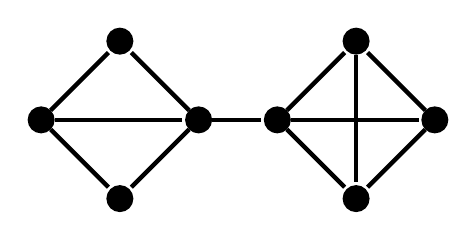
\begin{tikzpicture}[shorten >=1pt, auto, node distance=3cm, ultra thick,main node/.style={circle,fill=black,draw,minimum size=.1cm,inner sep=0pt]}]%
\begin{scope}%[every node/.style={font=\sffamily\Large\bfseries}]%[main node]
\node[main node] (v1) at (0,0) {1};
\node[main node] (v2) at (2,0) {2};
\node[main node] (v3) at (1,1){3};
\node[main node] (v4) at (1,-1){4};
\node[main node] (v5) at (3,0) {5};
\node[main node] (v6) at (5,0) {6};
\node[main node] (v7) at (4,1) {7};
\node[main node] (v8) at (4,-1) {8};
\end{scope}
\begin{scope}[every edge/.style={draw=black,ultra thick}]
\draw  (v1) edge (v2);
\draw  (v1) edge (v3);
\draw  (v1) edge (v4);
\draw  (v2) edge (v3);
\draw  (v2) edge (v4);
\draw  (v2) edge (v5);
\draw  (v5) edge (v6);
\draw  (v5) edge (v7);
\draw  (v5) edge (v8);
\draw  (v6) edge (v7);
\draw  (v6) edge (v8);
\draw  (v7) edge (v8);
\end{scope}
\end{tikzpicture}
\caption*{Graf $G$ posiadający dwie kliki o wielkości 3 oraz klikę wielkości 4, czyli $\omega (G) =4$ }
\end{figure}
\end{description}



\subsection{Programowanie liniowe}
\begin{definition}[Silne twierdzenie dualności]
$$\max _{\bar{x}}f(\bar{x})=\min _{\bar{y}}g(\bar{y})$$
\end{definition}
\begin{problem*}[Znaleźć maksimum funkcji $f$]
\begin{align*}
&f(x_1,x_2,x_3)=6x_1+4x_2+x_3\\
&\left\{\begin{matrix}
3x_1 &+	2x_2 &+	x_3 &\leq 8\\
1x_1 &+	2x_2 &+	x_3 &\leq 5\\
1x_1 &+	0 &		x_3 &\leq 1\\
x_1, &	x_2, &	x_3	&\geq 0
\end{matrix}\right.\\
&\begin{matrix}
y_1:3x_1 &+	2x_2 &+	x_3 &\leq 8\\
y_2:x_1 &+	2x_2 &+ x_3 &\leq 5\\
y_3:x_1 &+		 &  x_3 &\leq 1
\end{matrix}\\
&\text{ZNALEĆ MINIMUM FUNKCJI FUNKCJI }g\\
&\left\{
\begin{matrix}
3y_1	&+ y_2	&+ y_3	&\geq 6\\
2y_1	&+ 2y_2	&& \geq 4\\
y_1		&+ y_2	&+ y_3	&\geq 1\\
y_1,	& y_2,	& y_3	&\geq 0
\end{matrix}
\right.\\
&\max _{x_1x_2x_3} f(x_1,x_2,x_3)\leq \min _{y_1y_2y_3} g(y_1,y_2,y_3)\\
&\text{ dla }y_1=0,\ y_2=2,\ y_3=4\\
&\min _{y_1y_2y_3} g(y_1,y_2,y_3)=14\\
&\text{ dla }x_1=1,\ x_2=2,\ x_3=0\\
&\max _{x_1x_2x_3} f(x_1,x_2,x_3)=14
\end{align*}
\end{problem*}

\begin{problem*}[Znaleźć maksimum funkcji $f$]
\begin{align*}
&f(\bar{x})=\bar{c}^T \bar{x}\\
&\text{przy ograniczeniu: }\\
&A\bar{x}\leq \bar{b}\\
&\bar{x} = \begin{bmatrix}
x_1\\x_2\\x_3
\end{bmatrix} & \bar{c}^T = \begin{bmatrix}
6&4&1
\end{bmatrix}\\
&A=\begin{bmatrix}
3&2&1\\1&2&1\\1&0&1
\end{bmatrix} & \bar{b}=\begin{bmatrix}
8\\5\\1
\end{bmatrix}
\end{align*}
Znaleźć minimum funkcji $g$
$$g(y)=b^Ty$$
przy ograniczeniach
\begin{align*}
&A^T\bar{y}\geq \bar{c}\\
&\bar{y} \geq 0
\end{align*}
\end{problem*}

\begin{theorem}
Jeśli $x^\star$ maksymalizuje po $f(x)$ a $y^\star$ minimalizuje po $g(y)$ wtedy:
$$f(x^\star)=c^Tx^\star =b^Ty^\star =g(y^\star)$$
\end{theorem}

\subsection{Ułamkowe charakterystyki grafów}
\begin{definition}[$\beta (G)$]
Niech $G$ będzie grafem o $n$ wierzchołkach i $m$ krawędziach.\\Niech $\beta (G)$ oznacza wielkość największego skojarzenia w grafie.
\end{definition}

\begin{figure}[H]
\centering
\begin{minipage}{.5\textwidth}
\centering
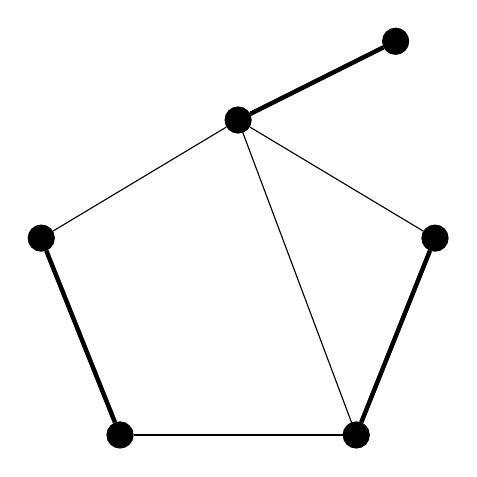
\begin{tikzpicture}[every node/.style={circle, draw, minimum size=0.05cm,fill=black}]
\node (v1) at (2,1) {};
\node (v2) at (0,0) {};
\node (v6) at (-2.5,-1.5) {};
\node (v3) at (2.5,-1.5) {};
\node (v5) at (-1.5,-4) {};
\node (v4) at (1.5,-4) {};
\draw[ultra thick]  (v1) edge (v2);
\draw  (v2) edge (v3);
\draw  (v2) edge (v4);
\draw[ultra thick]  (v3) edge (v4);
\draw  (v4) edge (v5);
\draw[ultra thick]  (v5) edge (v6);
\draw  (v6) edge (v2);
\end{tikzpicture}
\caption*{$\beta (G)=3$, $\gamma (G)=3$}
\end{minipage}%
\begin{minipage}{.5\textwidth}
\centering
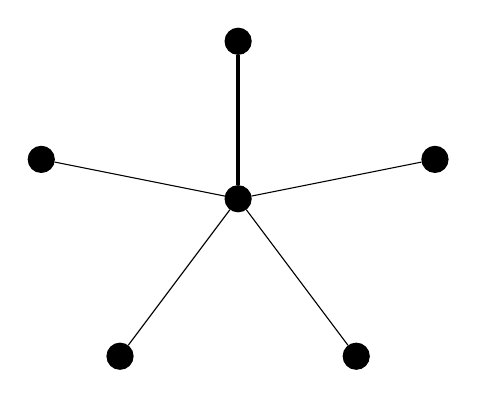
\begin{tikzpicture}[every node/.style={circle, draw, minimum size=0.05cm,fill=black}]
\node (v1) at (0,-2) {};
\node (v2) at (0,0) {};
\node (v6) at (-2.5,-1.5) {};
\node (v3) at (2.5,-1.5) {};
\node (v5) at (-1.5,-4) {};
\node (v4) at (1.5,-4) {};

\draw[ultra thick]  (v2) edge (v1);
\draw  (v1) edge (v3);
\draw  (v4) edge (v1);
\draw  (v1) edge (v5);
\draw  (v6) edge (v1);
\end{tikzpicture}
\caption*{$\beta (G)=1$, $\gamma (G)=1$}
\end{minipage}
\end{figure}

\begin{definition}[$\beta ^\star (G)$]
Dla każdej krawędzi $C\subseteq G$ wprowadzamy zmienną $x_C$ taką, że $x_C=1$ gdy $e$ należy do skojarzenia, a $x_e=0$ gdy nie należy do skojarzenia:
$$f(x_1,\dots x_n)=\sum _{c\in E}x_c$$
($x_c$ $\rightarrow$ wartości na krawędziach) dla każdego wierzchołka $v$ 
$$\forall _v \sum _{v\in e}  x_e \leq 1$$
\begin{align*}
&x_e \in \xcancel{\{0,1\}}\\
&0\leq x_e\leq 1\\
&\beta ^\star (G)\ \rightarrow \text{ułamkowa liczba skojarzenia grafu}
\end{align*}
\end{definition}

\begin{fact}
$$\beta ^\star (G)\geq \beta (G)$$
\end{fact}

Dla każdego wierzchołka wprowadzamy zmienną $y_v$.\\Będziemy szukali minimum następującej funkcji
\begin{align*}
&g(y_1,\dots y_n)=\sum _{v\in V}y_v\\
&\forall _{\begin{matrix}
e\in E\\e\in\{v,w\}
\end{matrix}} y_v+y_w\geq 1\\
&y_v=[0;1]
\end{align*}
\begin{definition}[$\gamma (G)$]
Minimalna liczna pokryciowa $\gamma (G)$, to najmniejsza liczba wierzchołków w zbiorze $w\subseteq V$ takim, że każda krawędź ma przynajmniej jeden koniec w $w$.
\end{definition}

\begin{fact}
$$\gamma (G) \geq \beta (G)$$
\end{fact}
\begin{fact}
$$\gamma (G) \geq \gamma ^\star (G)$$
\end{fact}
\begin{fact}
$$\gamma (G) \geq \gamma ^\star (G)=\beta ^\star (G)\geq \beta (G)$$
\end{fact}

\begin{example*}
przykład:
\begin{figure}[H]
\centering
\begin{minipage}{.5\textwidth}
\centering
\begin{tikzpicture}%[main node/.style={circle, draw, minimum size=0.05cm,fill=black}]
\node (v2) at (0,0) {};
\node (v6) at (-2.5,-1.5) {};
\node (v3) at (2.5,-1.5) {};
\node (v5) at (-1.5,-4) {};
\node (v4) at (1.5,-4) {};
\draw  (v2) edge node[above] {$\sfrac{1}{2}$} (v3);
\draw  (v3) edge node[above] {$\sfrac{1}{2}$} (v4);
\draw  (v4) edge node[above] {$\sfrac{1}{2}$} (v5);
\draw  (v5) edge node[above] {$\sfrac{1}{2}$} (v6);
\draw  (v6) edge node[above] {$\sfrac{1}{2}$} (v2);
\end{tikzpicture}
\caption*{$\beta ^\star (G)\geq 2.5$}
\end{minipage}%
\begin{minipage}{.5\textwidth}
\centering
\begin{tikzpicture}[every node/.style={above,draw}]
\node (v2) at (0,0) {$\sfrac{1}{2}$};
\node (v6) at (-2.5,-1.5) {$\sfrac{1}{2}$};
\node (v3) at (2.5,-1.5) {$\sfrac{1}{2}$};
\node (v5) at (-1.5,-4) {$\sfrac{1}{2}$};
\node (v4) at (1.5,-4) {$\sfrac{1}{2}$};
\draw  (v2) edge (v3);
\draw  (v3) edge (v4);
\draw  (v4) edge (v5);
\draw  (v5) edge (v6);
\draw  (v6) edge (v2);
\end{tikzpicture}
\caption*{$\gamma ^\star (G)\leq 2.5$}
\end{minipage}
\end{figure}
$$\beta ^\star =\gamma ^\star$$
\end{example*}

Oczywiście:
$$\beta (G)\leq \floor{\frac{n}{2}}$$

\textbf{Zadanie:} Uzasadnij, że $$\beta ^\star (G) \leq \frac{n}{2}$$
\begin{proof}
$$\beta ^\star (G)=\gamma ^\star (G) \leq \frac{n}{2}$$
Bo każdemu wierzchołkowi możemy dać wagę $\frac{1}{2}$.
\end{proof}

\begin{figure}[H]
\centering
\begin{minipage}{.5\textwidth}
\centering
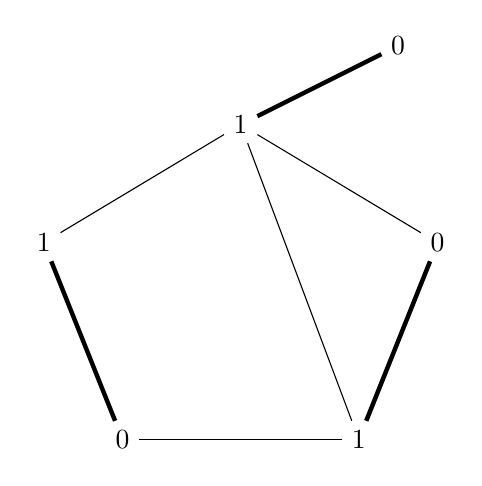
\begin{tikzpicture}%[every node/.style={circle, draw, minimum size=0.05cm,fill=black}]
\node (v1) at (2,1) {0};
\node (v2) at (0,0) {1};
\node (v6) at (-2.5,-1.5) {1};
\node (v3) at (2.5,-1.5) {0};
\node (v5) at (-1.5,-4) {0};
\node (v4) at (1.5,-4) {1};
\draw[ultra thick]  (v1) edge (v2);
\draw  (v2) edge (v3);
\draw  (v2) edge (v4);
\draw[ultra thick]  (v3) edge (v4);
\draw  (v4) edge (v5);
\draw[ultra thick]  (v5) edge (v6);
\draw  (v6) edge (v2);
\end{tikzpicture}
\end{minipage}%
\begin{minipage}{.5\textwidth}
\centering
\begin{tikzpicture}%[every node/.style={circle, draw, minimum size=0.05cm,fill=black}]
\node (v1) at (2,1) {};
\node (v2) at (0,0) {};
\node (v6) at (-2.5,-1.5) {};
\node (v3) at (2.5,-1.5) {};
\node (v5) at (-1.5,-4) {};
\node (v4) at (1.5,-4) {};
\draw  (v1) edge node[above] {1} (v2);
\draw  (v2) edge node[above] {0} (v3);
\draw  (v2) edge node[above] {1} (v4);
\draw  (v3) edge node[above] {1} (v4);
\draw  (v4) edge node[above] {0} (v5);
\draw  (v5) edge node[above] {1} (v6);
\draw  (v6) edge node[above] {0} (v2);
\end{tikzpicture}
\end{minipage}
\end{figure}

\begin{theorem}[D. Konig 1931]
Dla grafów dwudzielnych:
$$\begin{array}{ccc}
\beta (G) & = & \gamma (G) \\
\parallel &   & \parallel \\
\beta ^\star (G) & = & \gamma ^\star (G)
\end{array}$$
\end{theorem}

\begin{definition}[$\omega ^\star (G)$]
Ułamkową liczbą klikową $\omega ^\star (G)$ nazywamy maksymalną wartość funkcji:
$$f(x_1,\dots x_n)=\sum _{v\in V} x_v$$ 
przy czym dla każdego zbioru niezależnego $I$
\begin{align*}
&\sum _{v\in I} x_v\\
&x_v\geq 0\ \ x_v\in \{0,1\}
\end{align*}
\end{definition}

\begin{definition}[Ułamkowa liczba chromatyczna $\chi ^\star (G)$]
Każdemu zbiorowi niezależnemu $I$ przyporządkowujemy zmienną losową $y_I$ i minimalizujemy: $$\sum _I y_I$$ przy ograniczeniu, że 
\begin{align*}
&\forall _{v\in V} \sum _{\{I:v\in I\}}y_I\geq 1\\
&y_I\geq 0\\
&\text{dla }\chi (G) \text{ będzie } y_I=\{0,1\}
\end{align*}
\end{definition}

\begin{fact}
$$\chi (G)\geq \chi ^\star(G)=\omega ^\star(G)\geq \omega (G)$$
\end{fact}

\begin{figure}[H]
\centering
\begin{tikzpicture}%[main node/.style={circle, draw, minimum size=0.05cm,fill=black}]
\node (v2) at (0,0) {$v_1$};
\node (v6) at (-2.5,-1.5) {$v_5$};
\node (v3) at (2.5,-1.5) {$v_2$};
\node (v5) at (-1.5,-4) {$v_4$};
\node (v4) at (1.5,-4) {$v_3$};
\draw  (v2) edge (v3);
\draw  (v3) edge (v4);
\draw  (v4) edge (v5);
\draw  (v5) edge (v6);
\draw  (v6) edge (v2);
\end{tikzpicture}
\end{figure}
\begin{align*}
&v_1=v_2=v_3=v_4=v_5=\frac{1}{2}\\
&\text{zbiory niezależne: } 
\underset{\sfrac{1}{2}}{\{v_1,v_3\}}, \underset{\sfrac{1}{2}}{\{v_2,v_4\}},
\underset{\sfrac{1}{2}}{\{v_3,v_5\}}, \underset{\sfrac{1}{2}}{\{v_4,v_1\}},
\underset{\sfrac{1}{2}}{\{v_5,v_2\}}\\
&\chi (G)=3 & \omega (G) = 2\\
&\chi ^\star(G)\leq \sfrac{5}{2} & \omega ^\star(G)\geq \sfrac{5}{2}\\
&\chi ^\star(G) = \omega ^\star(G)= \sfrac{5}{2}\\
&\text{Ta własność } \chi (G)=\omega (G) \text{ jest bardzo rzadka wśród grafów}
\end{align*}





\end{document}
